\chapter{Economic and spatial concepts \label{chapter:location}}

\section{Introduction \label{sec:econsintro}}

%This chapter describes the elements used in the thesis model approach. The focus will be on the ideas that have been directly used in the models or arguments later on. It does this in two sections. The first outlines the key economic concepts of utility and production. The second looks at the following broader concepts: externalities, market structure and the `ecological criticism' of the production function approach.
%It also puts these in the wider context of spatial economics. In doing this, it also describes concepts that have been deliberately placed outside the scope of the model framework. 
This chapter outlines the economic and spatial concepts central to the thesis model framework. Section \ref{sec:econconceptsintro} begins laying out the foundation for the thesis model approach by explaining the utility and production functions that are used. The economic concepts in the thesis model framework have a strong connection to those used in \gls{ge}. The \gls{lov} utility function is central to the thesis, providing agents with a generic way of demanding goods across space while being able to control the mix of that demand. Instead of using the \gls{ge} approach to production, however, a different function is used that allows the transmission belt model to successfully link supply and demand and move between production equilibria.
%\gls{ge} has a strong claim to being the modern \emph{heir presumptive} of classical location theory: it has aimed to address 

Later sections introduce spatial economic ideas. These begin in section \ref{sec:spacesituate} by combining an overview of the `big questions' of spatial economics with an examination of the particular way that \gls{ge} has approached these problems and the role that dependencies and assumptions play. This section also discusses a number of other classical location theory ideas relevant to the models presented in sections \ref{sec:results} and \ref{sec:mobFirms}.

Section \ref{sec:coremodel} explains the \gls{coremodel} of \gls{ge} in detail, with the aim of carefully disassembling its `engine' and laying its parts out in a logical order. The purpose of disassembling the \gls{coremodel} is to aid the comparison of model-building methodology - and also philosophy - between \gls{ge} and \gls{abm}. Chapter \ref{chapter:ABM} concentrates on the more philosophical side of this problem and discusses the tendency of much \gls{abm} to be rather too literal in its interpretation of engine-building. 
%The second model results chapter (\ref{chapter:connectedModels}) examines a novel approach to linking supply and demand in agent form, informed by this comparison process.

After this, sections \ref{sec:elementsmodel} and \ref{sec:extsinspace} present context for the choices made in the thesis model framework. These are based on breaking down the catch-all term `space costs' into two elements: `distance costs' (the costs of moving people and goods across space; section \ref{sec:elementsmodel}) and the `costs and benefits of proximity'  (section \ref{sec:extsinspace}): that things being nearer to each other may be both beneficial or detrimental to them in ways pure distance costs cannot capture. 

The chapter ends with an outline of the concepts that have been deliberately placed outside the scope of the model framework. This sets up the discussion for `strategic simplifications' in the following chapter.

\section{Fundamental economic concepts \label{sec:econconceptsintro}}

\subsection{Factors \label{sec:factors1}}

At the most fundamental level, economic action is all about exchanging factors for other factors. Factors are often defined as broad abstractions. The most traditional of these is to identify capital ($K$) and labour ($L$) as the two inputs into aggregate production, where capital is a catch-all term variously meaning everything from factory plant to finance (\citealt{robinson_measure_1971} p.597). Arguments abound about the validity of this; some are discussed in chapter \ref{chapter:ABM}. The abstraction most common to \gls{ge} is to separate manufacturing ($M$) from agriculture ($F$), although, as will be explained, the distinction comes down to which sector has \gls{increts} and which is the unchanging base for comparison as values change.

The utility and production functions outlined below allow people and firms to get the most out of the factors at their disposal\footnote{It is an axiomatic economic idea that actors want to do this, though not a problematic one. This is discussed in section \ref{sec:produtility_agents}.}. 

The most important point to start with is that actors' time is given prominence. In \gls{ge}, this is equivalent to the labour they put into production. Section \ref{sec:ecocrit} looks at one particular critique of the way factors are treated in economics. The next section's outline of the utility functions used in the thesis will explain in more detail how factors are used.

\subsection{Utility \label{sec:utilityintro}}

%\cmt{Huh: just reading the very first introduction to utility in ch.2: it needs a rewrite, ideally, in the light of what we're doing with the core model. And some clarifying. E.g. I'm making the point that Cobb Douglas allows inc rets - but they're not used in GE. The CD is used because it keeps the two spends independent. That's the important feature. Need to get that in there.}
At its simplest, utility is a very effective way of describing when an economic actor is better or worse off. It can abstract away from any details about the nature of `better off' in any psychological sense. This is a strength of utility theory, though it is often portrayed as a weakness. Chapter \ref{chapter:ABM} examines these arguments in more depth, since they impact on the way that agent modellers have chosen to approach economics. 

As with \gls{ge}, the forms of utility used here are all reasonably simple and tractable. The simplest of these is the Cobb Douglas. A consumer gets utility from two goods, labelled $F$ and \textbf{$M$.} (For consistency, the variable names here are the same as those used later when discussing geographical economics.)

\begin{equation}
U=F^{a}M^{b}\label{eq:-1}
\end{equation}

The sum of $a$ and \textbf{$b$} control the effect of scale. Summing the exponents to one gives constant returns to scale, whereas if $a+b>1$, the function has \gls{increts}: increasing the amount of $F$ and/or $M$ causes a greater than proportional increase in utility (see section \ref{sec:prodfuncts} for a full explanation). Most commonly it is assumed that, for utility, $a+b=1$. For this, an equivalent function can be used:

\begin{equation}
U=F^{\delta}M{}^{1-\delta},(0<\delta<1)\label{eq:-3}
\end{equation}

This Cobb Douglas is particularly popular because of the convenient relationship that exists between a consumer's budget and the optimal mix of $F$ and \textbf{$M$. }Let $Y$ be the consumer's budget. Assuming the cost of both $F$ and \textbf{$M$} is unity (they both have a price of one), total consumption cannot be more than the budget:  

\begin{equation}
F+M=Y\label{eq:-2}
\end{equation}

What, then, is the optimal mix of the two goods for the consumer? Maximising \ref{eq:-3} with the budget constraint \ref{eq:-2} gives -

\begin{equation}
F=\delta Y\label{eq:cobbd_optF}
\end{equation}


\begin{equation}
M=1-\delta Y\label{eq:cobbd_optM}
\end{equation}

\begin{figure}[h]%
\centering
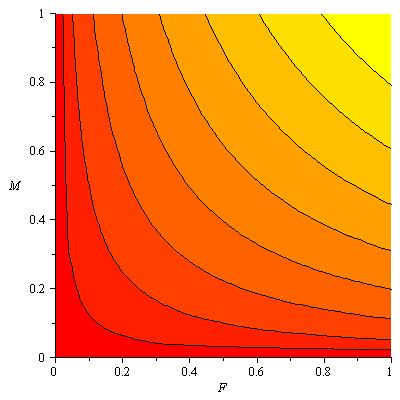
\includegraphics[width=0.7\columnwidth]{ChapterEcon/figures/cobbdouglascontour}%
\caption{Cobb Douglas function, $\delta$ is $0.5$. Contour lines show isoquants. Lighter colours are higher utility values.}%
\label{fig:cobbdouglascontour}%
\end{figure}

The Cobb Douglas exhibits, in the simplest way possible, a basic feature used by \gls{ge}: \gls{lov} - a mix of the two goods is preferable to either good alone; see below for a fuller description of this concept. The optimum mix can be controlled with $\delta$, which can be referred to as the `share parameter'. Figure \ref{fig:cobbdouglascontour} shows contour lines when $\delta=\frac{1}{2}$, indicating isoquants: lines of equal utility, where a consumer would be indifferent between the mix of $F$ and $M$, if their budget didn't matter. However, the budget does: according to \eqref{eq:cobbd_optF} and \eqref{eq:cobbd_optM}, their optimal choice if $\delta=\frac{1}{2}$ is equal. That is, $F=M$ - a positive, straight line. So, for example, if the budget $Y=10$, their utility-maximising mix would be five for each good. These preferences would also be homothetic - if the budget changes, the proportionate mix of optimal goods remains the same: $F$ always equals $M$. 
%(For a fuller outline of constrained optimisation for this and other functions in this section, see appendix \ref{apx:maths}.)

The strength of this simple function, then, is that $\delta$ can so easily be used to find the optimal mix of two goods given any budget. The next section looks at a slightly altered Cobb-Douglas where income level does matter.

\subsection{The CES function and `love of variety' \label{sec:CESbasics}}

%Three identical meals in a row for lunch and dinner is likely to be less satisfying than a good lunch and a three course dinner. 
The \gls{ces} function, and the economic ideas it represents, are used heavily throughout the thesis. \Gls{lov} and \gls{eosub} are two sides of the same coin: a few moments on the intuition of what they represent will help. If goods are completely substitutable (and thus have the highest possible \gls{eosub}) consumers will not mind which they have: each gives them the same utility. As \gls{eosub} drops, however, \gls{lov} comes into play: they increasingly prefer a mix of goods to a smaller range (while consuming the same overall quantity). At a very different scale, consumers prefer - in aggregate - a choice between (for example) four models of car than two, though in total they buy the same number of cars. (This example is returned to in section \ref{sec:coremodel}.) To the extent that consumers prefer a mix, they have high \gls{lov} and low \gls{eosub}. The more indifferent they are between goods, the higher the \gls{eosub} and the lower the \gls{lov}.

The \gls{ces} function is able to represent this dynamic with one parameter. First defined by Arrow et al. (\citealt{arrow_capital-labor_1961}), it is central to \gls{ge}. It is an economic swiss army knife; ``perhaps the most frequently employed function in modern economic analysis'' (\citealt{durlauf_new_2008} p.737) and is used to represent both production output and utility. The first appearance of the CES function, in its two-input form, saw it being applied to cross-country data. Dixit and Stiglitz give a clear illustration of the basic principle, using a function able to reflect that:

\begin{quote}
``... a consumer who is indifferent between the quantites $(1,0)$ and $(0,1)$ of two commodities prefers the mix ($\frac{1}{2},\frac{1}{2}$) to either extreme.'' (\citealt{dixit_monopolistic_1977} p.297)
\end{quote}

It is easiest to see how this works in a simple two-good function that looks like Dixit and Stiglitz's example, before moving on to the $n$-good case. Consider a consumer with the utility function: 

\begin{equation}
U=\left[F^{\rho}+M^{\rho}\right]^{1/\rho}\label{eq:-4}
\end{equation}

The first thing to note is that, if we suppose $M=0$, and only $F$ has a positive value, then $U=(F^{\rho})^{1/\rho}$. This is always just $U=F$, regardless of the value of $\rho$. If both goods have positive values, and $\rho=1$, this reduces to $U=F+M$ and utility is also entirely linear. But for $0<\rho<1$, the consumer is increasingly better off with a mix of the two goods as $\rho\rightarrow0$. So, for example, let $F=4$ and $M=4$. If $\rho=1,$this means utility is just 8. If $\rho=\frac{1}{2}$, however, $F$ and $M$ both become $2$. So utility is then $(2+2)^{2}$or 16 - double the linear result. In effect, $\rho$ is the \gls{lov}. For values of $0<\rho<1$, the two goods are imperfect substitutes. This can be seen if \eqref{eq:-4} is altered slightly to:

\begin{equation}
U=\left[\delta F^{\rho}+(1-\delta)M^{\rho}\right]^{1/\rho}\label{eq:-5}
\end{equation}

Again, $\delta$ is a share parameter, a built-in budget, and the consumer must choose a limited mix of the two goods. Figure \ref{fig:CEStwogoodconstrained} gives an example of the function with an equal amount of each good at the two extremes (four), spreading the share between the two. $\rho$ is $0.5$. This underscores Dixit and Stiglitz's basic point: four of either good alone gives less utility than an even mix, two of each.

%(section \ref{sec:constrainedopt} in appendix \ref{apx:maths} gives a more formal derivation showing that the optimal mix is always an even split between the two goods.)
%\cmt{The Cobb Douglas is a special case of the CES where $\rho=0$. Which is true, but not really easily seen: requires l'opital's rule. Should I mention it?}
There is also only one unique maximum for $\delta$, at 0.5. A consumer is best off with a perfect mix of the two, rather than either extreme. This is just a restatement of Dixit and Stiglitz's original point; however the simple principle illustrated here holds for all other versions of the CES. 


\begin{figure}%
\centering
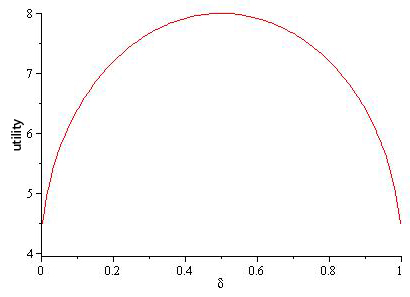
\includegraphics[width=0.7\columnwidth]{ChapterEcon/figures/CEStwogoodstradeoff2}%
\caption{Two-good CES function, $\rho=\frac{1}{2}$, constrained by $\delta$, $0<\delta<1$}%
\label{fig:CEStwogoodconstrained}%
\end{figure}

The many-good CES is just an extension of the above: 

\begin{equation}
U=\left(\sum_{i=1}^{N}c_{i}^{\rho}\right)^{1/\rho}\label{eq:-6}
\end{equation}

In this version, $c$ denotes the quantity of good $i$ and can be set individually, so that utility is dependent on all goods. (This is a feature of the \gls{ces} put to good use in the thesis model framework.) The continuous-varieties version of the \gls{ces} function is discussed in section \ref{sec:coremodel} in the context of the \gls{coremodel}. The next section outlines how these utility functions can be combined with budget constraints.

\subsection{Constrained optimisations \label{sec:constrained}}

A Lagrange multiplier is used to constrain a utility function by a budget equation. The essential point is that utility and budget equations are superseded by a third that describes demand for goods, given an actual budget amount and a set of goods prices. 
%(Appendix \ref{apx:maths} runs through the details of arriving at these constraints.)

Actors with a Cobb Douglas utility function \eqref{eq:-3} want to buy a mix of two goods $F$ and $M$, where $p_F$ and $p_M$ are the price of $F$ and $M$ respectively. The constrained optima including price are as follows:

\begin{equation}
F=\frac{\delta Y}{p_F}
\label{eq:optCDF}
\end{equation}
 
\begin{equation}
M=\frac{(1-\delta) Y}{p_M}
\label{eq:optCDM}
\end{equation}

%%%
% NO ENGEL FUNCTION
%%%
\begin{comment}
The constrained optima for the Engel function, \eqref{eq:EngelpriceoptM} and \eqref{eq:EngelpriceoptF}, reduce to the Cobb Douglas when $\gamma$ is zero. 

\begin{equation}
M=\frac{Y(1-\delta)}{p_{M}}-\delta\gamma
\label{eq:EngelpriceoptM}
\end{equation}
 
\begin{equation}
F=\frac{\delta Y-Y+\delta\gamma p_{M}}{p_{F}}
\label{eq:EngelpriceoptF}
\end{equation}
\end{comment}

For the \gls{ces} function, a constrained optimum can be defined for each single good, given a budget and the cost of each good. The optimal amount for good $g_j$ is given by:

\begin{equation}
g_j = \frac{P_j^\frac{1}{\rho-1}Y}{\sum_{i=1}^{n}P_i^\frac{\rho}{\rho-1}} \label{eq:CESconstrained}
\end{equation}

- where $p_j$ is the price of good $c_j$, $Y$ is the budget, and the denominator sums the price of each good raised to $\rho/\rho-1$. (Capital $P$ is used later for distinguishing the full good price including space costs from its base price, lower-case $p$.)\footnote{This single-good optimum was derived from Brakman \emph{et al.}'s constraint of a \gls{ces} function for a single good by substituting the price index back in and rearranging. See \citealt{brakman_new_2009} pp.94.}

\subsection{`Increasing returns' and production \label{sec:prodfuncts}}

%This thesis uses only the simplest production function: it has one input and one output. This is the same as the \gls{coremodel}, where labour is the only productive factor. 
The concept of \gls{increts} describes all economic situations where \emph{per-unit} output is higher for each extra amount of input (so where the first derivative of output with respect to input is always more than zero). In this thesis, \gls{increts} in \emph{production} are called \gls{eos} to distinguish them from \gls{increts} in utility as described by the \gls{ces} function. The relevance of this distinction is explained in section \ref{sec:ecocrit}. This section explains how \gls{increts} enter into production functions.
%The vital requirement for getting firms to function in space is economies of scale, or \gls{increts}. 
%For a Cobb Douglas-type function, the simple way to control returns to scale has already been mentioned: whether the sum of the exponents is more or less than one will dictate whether it exhibits increasing or diminishing returns respectively. 
%The most obvious multi-input function has already been mentioned in section \ref{sec:utilityintro}: the Cobb Douglas first came into being as a production function. 

Single-input production functions can use simple equation forms for turning an input into some larger output quantity. The \gls{coremodel} uses a straight line equation, where output ($x$) is defined in terms of the amount of labour ($l$) required to produce it, and where $\alpha$ are fixed costs and $\beta$ are marginal costs (see the next section for an outline of the use of `marginal'):

\begin{equation}
l = \alpha + \beta x
\label{eq:coremodelMprod}
\end{equation}}

%Setting $a=3$ and b to unity, and isolating the expression for the output, $x$, this becomes $x=l-3$.
Usually, `average labour' is the focus (which is labour per unit of output; this declines as total labour increases in \gls{increts} functions.) For the purposes of this discussion, it is easier to see the role that $\alpha$ - the fixed labour requirement - takes if instead the axes are switched and output is the focus:

\begin{equation}
x = \frac{l-\alpha}{\beta}
\end{equation}

The production function used in the thesis model framework also takes in a single input - people's time (or `labour'; these two terms refer to the same thing here). Many different people can input into a single firm, increasing its production efficiency. Section \ref{sec:abmprod} sets out how this is done in the framework. However, due to vital differences between agent modelling and the analytic approach represented by the \gls{coremodel} (also outlined in section \ref{sec:abmprod}), the function used is of a different form. 

The production function used in the thesis is `smooth': it does not have a fixed and marginal component, but instead a nonlinear and linear component, each separately scalable. To achieve the small increase in productivity per unit of input time required, a nonlinear increment to linear production is added as labour input increases, such that the second derivative of the function is positive (it is zero in the \gls{coremodel}'s production function). The basic version is this:

\begin{equation}
x=l+l^{2} \label{eq:smoothEoS}
\end{equation}

In the thesis models, each of the two terms is given its own parameter as a way to control scale in particular model runs:

\begin{equation}
x=m l+ v l^{2}\label{eq:smoothEoS2}
\end{equation}

-	where $v$ is the `curve' parameter controlling the scale of returns and $m$ is the magnitude of the linear component. This gives a simple smooth curve increasing output per unit of labour input as labour goes up. 

\begin{figure}
  \centering
  \subfloat[core model style]
  {\label{fig:fixedIncRets}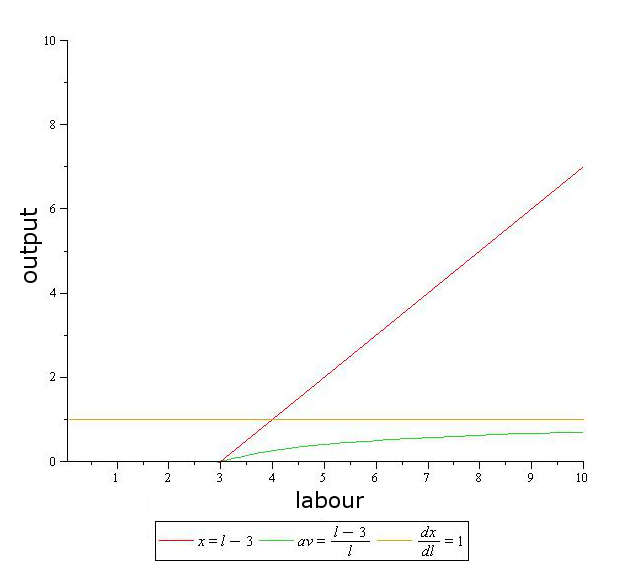
\includegraphics[width=0.75\textwidth]{ChapterEcon/figures/coremodelprodABM1edited}}
  \hspace{0.2}  
  \subfloat[smooth]{\label{fig:smoothIncRets}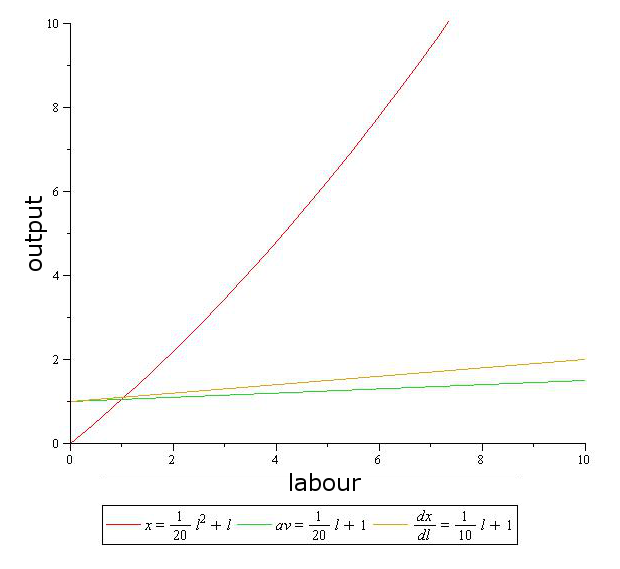
\includegraphics[width=0.75\textwidth]{ChapterEcon/figures/smoothIncRets1edited}}
  \caption{Two ways to achieve increasing returns for a single input. (a) core model style production function; (b) `smooth increasing returns' function. Both show total, average and marginal output per unit of labour.}
  \label{fig:incRetsFunctions}
\end{figure}

Figure \ref{fig:incRetsFunctions} graphs both the \gls{coremodel} production function (for $\alpha =3$ and $\beta = 1$) and the `smooth' \gls{eos} function (for $v = \frac{1}{20}$ and $m = 1$). Their different structure shows up: both marginal and average output increases for the smooth function (\ref{fig:smoothIncRets}). The version used in the \gls{coremodel} (\ref{fig:fixedIncRets}) is built on fixed and marginal quantities (see the following section) so it already has a constant marginal output built in. The only other difference is that average output for a unit of labour in the \gls{coremodel} increases, but at a decreasing rate (its second derivative is $-6/l^3$), whereas the smooth function's average increases constantly.

So does it matter which is used? In the analytic approach of the \gls{coremodel}, a fixed and marginal labour requirement makes sense, since they can both be treated algebraically (this is discussed further in section \ref{cmcomp}). In an agent model, however if a `fixed labour' amount is required, it needs to actually be supplied. This is not impossible, but it impacts directly on whether or not such a model functions correctly, given its set of components. The smooth \gls{eos} function allows for any amount of input to produce output; in contrast, the \gls{coremodel} function produces negative output for fixed labour values below $\alpha$. These issues are discussed in section \ref{sec:blindvsrational}, and models using these functions are discussed in section \ref{sec:prodtowelfare}.

\subsection{The meaning of `marginal' \label{sec:marginalapx}}

A quick note on terminology. Classical Economics has been described as the `marginal revolution'. The term `marginal' just means the first derivative of some quantity. Here is one example from utility and one from production. To start with the Cobb Douglas function discussed in section \ref{sec:utilityintro}: if one quantity is held constant, the other's diminishing marginal utility can be seen from graphing the partial derivative, $\frac{\partial U}{\partial f}=\frac{\sqrt{M}}{2\sqrt{F}}$ - see figure \ref{fig:dmu_cobbd}, where $M$ is set to one. The change in utility per unit diminishes (so $U''<0$); as more is consumed, each extra unit becomes less `satisfying'. Note, this makes sense given what has been said about the Cobb Douglas exhibiting basic `love of variety': if $M$ is held constant as $F$ increases, `variety' is actually dropping away from a perfect mix of the two.

\begin{figure}[h!]
\centering
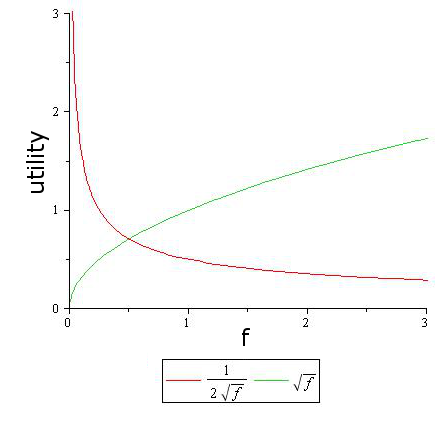
\includegraphics[width=0.6\columnwidth]{ChapterEcon/figures/DMU_cobbdouglasedited}%
\caption{Total ($\sqrt{f}$) and marginal ($1/2\sqrt{f}$) utility for a $\delta=\frac{1}{2}$ Cobb Douglas utility function, holding $M$ constant at 1. }%
\label{fig:dmu_cobbd}%
\end{figure}

As discussed, the same kinds of functions are used for firms and so the same principles hold. The canonical result for firms is that output should be set where marginal cost equals marginal revenue ($MC=MR$). This is a straightforward intuition: a firm increases output by one unit. If the extra cost is lower than the extra revenue, they can still make money. If the cost is higher than the extra revenue, they would lose money. So this directs them to the point where any change in cost exactly matches the change in revenue: $MC = MR$. For this to work, the firm's change in output cannot affect prices: see section \ref{sec:marketstructure}. 
%Section \ref{sec:dmr} explains why, in an agent model, it cannot be assumed firms `know' 
This completes the explanation of the utility and production functions used in the thesis model framework, though the nature of the assumptions involved and how the functions are used is discussed throughout the thesis.

\section{Bringing space into economics \label{sec:spacesituate}}

This section examines a set of key issues for understanding how spatial economics has been theorised and the form it has taken in \gls{ge}. The discussion is shaped by thinking about the assumptions and dependencies involved. Section \ref{sec:overview} gives an overview of the spatial economic `problem' and offers an initial thought regarding why \gls{abm} struggles with spatial economics, setting the scene for chapter \ref{chapter:ABM}. The following three sections explain the central market structure dependencies that determine what is considered a `valid' spatial economic explanation in \gls{ge}. Section \ref{sec:ecocrit} looks at the nature of the `\gls{increts}' assumption as context for understanding how \gls{lov} and \gls{eos} (two different forms of \gls{increts}) are treated separately in the thesis model framework.

\subsection{Overview \label{sec:overview}}
Spatial economics, both classical and modern, asks the broadest of questions about economic activity: ``who produces what, where and why?'' (\citealt{ohlin_interregional_1933} quoted in \citeauthor{brakman_new_2009}, p.81)  Spatial structure is one of the most obvious facts of economics, and one of the most difficult to explain. \citeauthor{duranton_micro-foundations_2003} (2003) put it well: ``Only 1.9\% of the land area of the United States was built up or paved by 1992. Yet, despite the wide availability of open space, almost all recent development is less than one kilometre away from earlier development.'' From the point of view of much economic theory, this shouldn't happen at all -

\begin{quote}``If we postulate only the usual list of economic forces, cities should fly apart. The theory of production contains nothing to hold a city together. A city is simply a collection of factors of production, capital, people and land - and land is always far cheaper outside cities than inside. Why don't capital and people move outside, combining themselves with cheaper land and thereby increasing profits?'' (\citealt{lucas_mechanics_1988} , p.38)
\end{quote}

\gls{ge} is the most prominent modern spatial economic theory to offer an answer. Paul Krugman, the original creator of the \gls{coremodel} at the heart of the method, asks, ``why and when does manufacturing become concentrated in a few regions, leaving others relatively undeveloped?'' (\citealt{krugman_increasing_1991}, p.484) The success of \gls{ge} stems from a framework able to address each of Ohlin's `what, where and why'. What is produced? A variety of generic products. The more variety, the better-off the consumers. Where is it produced? There is a `cumulative causation' between the location choice of firms and people. Combined with transport costs, the core model (section \ref{sec:coremodel}) claims to answer the `why' - a positive feedback flowing from the decisions of rational actors. The model shows how it is possible for one region, with no natural advantage, to end up a core producing area, while another is periphery.
%As section \ref{sec:coremodel} discusses in more depth, \gls{ge}'s approach relies on modelling the interaction between an internalised `iceberg' cost of transport between discrete regions, each internally a point economy, and the effect of externalities for those actors within each region. 

The \gls{coremodel} is such a vital point in the history of spatial economics because it connected `general' and `spatial' for the first time. This and the following sections explain why this was so important. Calls for a `general location theory' to parallel general equilibrium models in (non-spatial) neoclassical economics go back at least as far as Isard (\citealt{isard_location_1956}). For Isard, general equilibrium was a ``wonderland of no dimension'' (ibid p.26). In the period between Isard's and Krugman's work, however, general equilibrium continued to avoid explicit space. As Isserman notes (\citealt{isserman_its_1996}), Krugman repeated Isard's claim almost verbatim, pointing out that ``in the late nineteen-eighties mainstream economists were almost literally oblivious to the fact that economies aren't dimensionless points in space'' (\citealt{krugman_new_2010}, p.1).  

Krugman's stated aim in developing his model was to build a bridge between neoclassical economics and geography, precisely in order to encourage `dimensionless' neoclassical economists to take geography seriously. What was the bait used to lure neoclassical economists out of their dimensionless `wonderland' onto new geographical pastures? A model able to preserve all the key neoclassical features: a self-contained general equilibrium outcome reached through maximising utility, by building on his insights in trade theory that had used \gls{monocomp} to solve the `similar-similar problem' (\citealt{krugman_increasing_2009-1} p.561) of international trade in similar sectors (see section \ref{sec:cmstory}). As section \ref{sec:marketstructure} outlines, the vital element is provided by the new approach to market structure of the Dixit-Stiglitz method: the ability to construct a non-perfect-competition model, required by the neoclassical approach for allowing spatial economic activity to happen at all (see section \ref{sec:marketstructnspace} for more on this).
%In doing so, \gls{ge} linked two previously separate outcomes in a general equilibrium framework: geographical morphology and welfare. Actors attempting to find better utility produce specific spatial patterns. This also raised the possibility that welfare can equilibriate while producing radically different spatial outcomes; equally, welfare can change while morphology does not. 

The success of Krugman's project, however, throws into sharp relief the absence of other attempts to examine these fundamental components of spatial economics. This may be, as Overman notes (quoting Martin \citeyear{martin_new_1999}) that many see -

\begin{quote}
`` - individual optimising behaviour, equilibrium outcomes and mathematical modelling as a regressive step for economic geographers who have `long since abandoned location-theoretic and regional science models'.'' (\citealt{overman_can_2004}, p.505)
\end{quote}

The analytic approach of \gls{ge} is - as many \gls{ge} theorists openly acknowledge - a `mathematical straitjacket' (\citealt{martin_new_1999}). The difference between \gls{ge} and `economic geography proper' (as Martin puts it) is in their evaluation of whether the benefits of the straitjacket outweigh the costs. 

Martin argues that \gls{ge} is unable to properly explain the real internal dynamics that make localisation more productive. Many theorists agree with this while remaining ``squarely on the side of those who consider that general frameworks are necessary to scientific progress in geographic economics'' (Storper 2010 p.315). They want to be able to ``pinpoint the basic sources of urban dynamism, which lie in the selective geographical matching of productive resources, skills and institutions of coordination'' (\citealt{storper_rethinking_2009} p.164). Duranton and Puga have done just that, concentrating on the underlying microfoundational mechanisms of `sharing, matching and learning' taking place (\citealt{duranton_micro-foundations_2003}), as well as broadening out to investigate the ``conditions for a configuration in which diversified and specialized cities co-exist to be a steady state'' (\citealt{duranton_nursery_2001} p.1). See also more recently Delgado \emph{et al.} (\citeyear{delgado_clusters_2010}) for a subtle empirical look at the interaction of clustering, productivity and startups: ``while at a (narrow) industry level firms may compete for the given pool of resources, the cluster environment that surrounds an industry will increase the pool of competitive resources and reduce the barriers of entry for new firms'' (ibid p.514). 
%Storper, however, worries about leaving out the ``wider dynamics that shape the concrete opportunities for and limits on behaviour'' (\citealt{storper_rethinking_2009} p.165).
%The rest of this chapter explains the geographical ideas used in this thesis, as well as the strategic simplifications made.

Fowler argues that \gls{abm} is perfectly positioned to help ``bridge the gap between geographical economics and economic geography'' (\citealt{fowler_taking_2007} p.266; section \ref{sec:fowler}). However, agent modelling seems to have a default affinity with ``economic geography proper''s outright rejection of everything neoclassical (section \ref{sec:ace}), leaving \gls{ge} and \gls{abm} in quite incompatible positions. \gls{abm} also tends to chime with Martin's argument about \gls{ge}: that valid explanations require digging into a system's internal dynamics (section \ref{sec:levels}).
 
The rationale for `disassembling' the \gls{coremodel} in section \ref{sec:coremodel} is to gain the opportunity to carefully compare the assumptions of \gls{ge} and \gls{abm} in an attempt to question the validity of this common \gls{abm} rejection of everything neoclassical. The two cannot easily be directly translated into each other (as Fowler's work has revealed; section \ref{sec:fowler}) and each has very a different model assumption space. Laying these out clearly enables a more informed set of choices for building spatial ideas into the thesis model framework.
%As chapter \ref{chapter:ABM} discusses in more detail, it would not be too much of an exaggeration to say that the research agenda of \gls{abm} has been specifically about pursuing that rejection. 
%The following two sections explain the `dependencies' at the heart of economics that have determined how the spatial economy has come to be theorised. 

\subsection{Market structure \label{sec:marketstructure}}

%The way in which market structure has been theorised lies at the heart of how space has come to be modelled in \gls{ge} and why it has mostly been avoided in mainstream economics. 
This and the following section examine the `dependencies' at the heart of market structure arguments and explain how they have determined the role of space in economics. There are three broad categories of favoured market structure in analytic economics: perfect competition, monopoly and \gls{monocomp}. Why `favoured'? Each of these are analytically tractable, (relatively) simple and allow some strong economic conclusions to be drawn from static equilibrium analyses. The last of these - \gls{monocomp} - is vital to the `engine' of the \gls{coremodel} (section \ref{sec:coremodel}).
%and elsewhere and is the site at which `dependencies' clearly arise in more traditional economic theory. 


Perfect competition and monopoly have straightforward mathematical interpretations: in the former, the size of the market is so large that no one economic actor can affect price: everyone is assumed to be a `price-taker'. In practice this means prices can be treated as constants. (This is generally the case, though general equilibrium theory has developed an argument for perfect competition that does not rely on assuming all actors are price-takers; see e.g. \citealt{starr_general_1997} pp.157.) Not only does this mean consumers can have no effect on price, but firms cannot either - and so strategic interaction is ruled out. In a monopoly, on the other hand, the monopoly firm can set a price that gives them the best revenue, based on the supply-demand curve they face for their product. There are no other firms, so they face no strategic considerations, and the revenue-maximising calculation is straightforward.

Perfectly competitive models must work with linear output - no \gls{increts} are allowed. To see why, consider a (rather artificial) situation where many firms have linear output, but one firm, producing the same good, is able to utilise \gls{eos}. They can thus produce each unit more cheaply than their competitors - and so this is no longer a perfect competition situation. A single price can no longer be assumed, nor can one say that no actor can influence price. In this case, that firm can immediately affect demand for other firms' goods; the more goods are substitutable (in the \gls{ces} function, as $\rho \rightarrow 1$), the more monopoly power that firm can gain.

\Gls{increts} also create `indivisibilities': if a particular product can be produced more efficiently at a larger scale, there is no incentive to `divide' this productive capacity into smaller strands, each producing less efficiently. Those efficiency gains provides firms with market power. This idea is important for \gls{ge} and the \gls{coremodel}; it is used to justify individual firms producing a single variety and is the basis for its market structure argument (see section \ref{sec:CMproduction}).

Between these two poles, analyses of `imperfect competition' have produced a sprawling tangle of approaches over the twentieth century, with some famous early attempts at synthesis (e.g. \citealt{robinson_economics_1933}). The arrival of the \gls{dxs} is such a pivotal moment in the history of market structure models because it offered a (relatively) simple way of keeping a stylised form of imperfect competition while saying useful things about the economy as a whole. The \gls{monocomp} model first published by \citeauthor{dixit_monopolistic_1977} in 1977 is one of the most prominent approaches to imperfect competition. It is the `engine' of \gls{ge} (a description discussed in more depth in section \ref{sec:coremodel}). As Brakman \emph{et al.} note, in providing a tractable method able to do away with many of the complexities facing theorists of imperfect competition, it neatly sidesteps ``getting bogged down in a taxonomy of oligopoly models'' (\citealt{brakman_new_2009} p.93). In particular, it can account for economies of scale, and it finds a way around problems of strategic interaction. The workings of this `combustion engine' as it is applied to the \gls{coremodel} are explained in section \ref{sec:coremodel}.


\subsection{Preconditions for spatial economic activity \label{sec:marketstructnspace}}

The development of the \gls{coremodel} was motivated by the fact that previous economic theory, built on perfect competition models, was unable to deal with space. The problem begins with the relationship between perfect competition and \gls{increts} explained in the previous section. Perfect competition cannot work with \gls{increts}, because any firm able to gain them will have a cost advantage: that is immediately no longer perfect competition. It would also nix the possibility of assuming agents are price-takers and that there is one price. Economics in space, however, cannot work \emph{without} \gls{increts}, because if output is linear, gains from trading across space can never be enough to compensate for losses incurred transporting goods or people. This issue led to space being largely ignored by mainstream economics. As Fujita put it:

\begin{quote}
``since the traditional general equilibrium analysis abstains from the consideration of indivisibilities or \gls{increts}, it fails to capture the essential impact of transport and spatial costs on the distribution of economic activities.'' (\citealt{fujita_location_1999} p.376})
\end{quote}

The way in which perfect competition rules out spatial economic models has been dubbed the `spatial impossibility theorem' by Fujita. Starrett (1978) is credited with first making this point formally. As Fujita and Thisse describe it -

\begin{quote}
``Starrett has shown that if space is homogenous and transport costly, then... the economy degenerates into separate single-location groups of agents with all trades taking place within, rather than between, groups. Consequently, the perfectly competitive price mechanism alone is unable to deal simultaneously with cities and trade.'' (\citealt{fujita_economics_2002} p.13-14) 
\end{quote}

To put it another way: if an actor is able to produce `in their own backyard', why would they choose to trade or collaborate in a world where all producers' output is linear? Any gain they would receive can never outweigh transport costs. As a consequence, ``people in each of these locations, like Robinson Crusoe, will produce all goods at a small scale for self-consumption.'' (\citealt{duranton_micro-foundations_2003} p.1) However, with \gls{increts} introduced to the picture, the minimum conditions for spatial economic activity now exist. So \gls{increts} serve a dual purpose: they allow actors to break out of this `spatial impossibility' trap, as well as guaranteeing uniqueness of varieties due to creating indivisibilities (a vital assumption for the \gls{coremodel}; section \ref{sec:CMproduction}).

The overlap of market structure arguments and the preconditions for spatial economic activity are responsible for the key `dependencies' that have driven the development of economics and its separation, until recently, from spatial economics. \gls{ge} models are built to make sure space is not impossible: locations do not lapse into autarky, and economic activity does not collapse into a single point `black hole' (\citealt{fujita_location_1999} p.58). 

Through the use of an `iceberg' conception of trade costs (see section \ref{sec:cmtoplevelstructure}) the \gls{coremodel} also gets to use the \gls{dxs} while tactically avoiding the second key problem that space imposes: market interactions are ``not all brought together in a single location and at the same time'' (\citealt{leijonhufvud_agent-based_2006} p.1633). This simple fact about spatial trade breaks the assumption that exchanges happen in a centralised `auction' way: there is no single site where prices can equilibriate to `clear' supply and demand efficiently. For this reason alone, Isard argues, ``the generally accepted principle of pure competition is not applicable to the analysis of spatial economic processes'' (\citealt{isard_location_1956}  p.489-490). This point is taken up in more detail in section \ref{sec:ace} as something \gls{abm} is in theory primed for. 
%Note, however, this is a different argument to `incomplete competition' due to \gls{increts} or spatial impossibility. Isard is talking about something much more basic: space itself imposes those limitations. This point is discussed in more depth in section \ref{sec:ace}.

\subsection{Endogenisation \label{sec:endog}}

The drive towards `general' economic models is underpinned by arguments for `endogenising' economic dynamics into those models. Section \ref{sec:coremodel} explores one example of this, where the use of the \gls{dxs} provides an explanation of international trade that does not require any exogenous imposition of differences between countries. From this point of view, many classical location theories fall short, requiring many exogenous impositions to function; section \ref{sec:litbits} looks at a number of these relevant to the thesis models. 

\gls{ge} brings the same philosophy to spatial economics, seeking to model spatial morphology ``as an endogenous outcome of the economic process'' (\citealt{storper_agglomeration_2010}, p.315), rather than being caused by `first nature' effects, such as ``political power (the State), trade (rivers and ports), and finance'' (ibid p.316), or the presence of natural resources. These may determine starting conditions, but the goal is to identify and understand `second nature' effects - those that flow from the interaction of people and firms in space, not some external spatial feature. As Glaeser argues (\citealt{glaeser_cities_2004}, \citealt{glaeser_cities_2008} p.7), as transport costs decline, any exogenously imposed distance factors resulting from `first nature' landscape features decline relatively in importance. On this basis, Fujita argues that - 

\begin{quote}
``To test whether a model can explain the endogenous formation of agglomerations, it is best to consider the simplest case of a perfectly homogenous geographical space (and free choice of location by all agents), for if any concentration of economic activities occurs in such a homogenous space, it must be due to endogenous forces.'' (\citealt{fujita_location_1999} p.376-7)
\end{quote}

The need for increasing returns to allow spatial trade to happen at all also stems from the same motivation. Many older classical location theories (discussed in section \ref{sec:litbits}) breach the `spatial impossibility' condition by not explicitly modelling increasing returns, thus providing no endogenous motivation for trade to occur at all.

In the thesis models, the difference between an exogenous and endogenous model shows up in sections \ref{sec:LoVresult} and \ref{sec:tbmplusdensity}, which present two results where an exogenous difference in the first is found endogenously in the second, more `general' model. Partial models with exogenously fixed features still have their uses, however; chapter \ref{chapter:models} makes use of partial models to make specific points relevant to the thesis. The use of a `density cost' proxy in the models in section \ref{sec:results} is based on a particularly agent-based take on endogenisation, where all costs of being `here' are endogenised; this is discussed in section \ref{sec:1st2ndnature}. 

There is another potentially disruptive point mentioned in passing by Fujita at the end of his speech honouring Walter Isard in 1999:

\begin{quote}
``For the development of human society in the long-run, economic aspects represent merely a part of the phenomenon, perhaps not even the most important ones. In other words, economic development may represent merely a possible result of the more fundamental process of social and cultural development.'' (\citealt{fujita_location_1999} p.380)
\end{quote}

If, in reality, the spatial economy is a complex mix of economic and other factors, this may suggest this `endogenise everything' philosophy will always produce incomplete models if it relies on purely economic forces. This point is returned to in the conclusion. 

The previous sections suggest the following: an \gls{abm} `general' theory of spatial economics would require solving the following two problems. First, an effective market structure would be required, capable of allowing genuine competition dynamics, or at least developing a specifically \gls{abm}-friendly argument about competition. Second, there would need to be no imposed condition about when or where economic exchanges are initiated. Or, less strongly, economic exchanges would be required to avoid the need to happen at a single time and place, `auction' style (this last point is given a more detailed treatment in section \ref{sec:ace}).

The transmission belt model presented in chapter \ref{chapter:connectedModels} is the result of finding a series of modelling compromises in pursuit of this goal. It is most successful in producing  stable supply/demand equilibria for agents at differing locations, through decentralised price signals. There is no single auction site or process: equilibrium is the result of individual Firms' price signals responding to market signals from all People, with both Firms and People having heterogenous locations. However, it does this with no explicit competition dynamic between firms, even though they do use price adjustment to sell goods and effectively clear the market. The next chapter, in examining \gls{abm}, discusses how the kind of coordination issues involved in market structure problems have been a prominent research topic for \gls{abm}. Many problems still appear unresolved: this key point is returned to both in the chapter presenting the transmission belt model results and in the conclusion. 

\subsection{The `ecological' criticism \label{sec:ecocrit}}

%Ecol crit: I want to tie this directly to the core model, as well as my own: time into output? What actually is output in GE? Does it matter? Can we address that? Are we OK with e.g. combining other inputs? Anyway, this is the place to tie that in. Specifically talk about murkiness of core model's manufacturing 'composite', compare to the job it is being asked to do.
%Before coming onto the \gls{coremodel}, this section briefly examines a question about the nature of what is being produced in the kinds of economic models discussed above. 
The discussion of market structure in sections \ref{sec:marketstructure} and \ref{sec:marketstructnspace} explained that \gls{increts} are a vital component of the \gls{ge} rationale for spatial activity. As section \ref{sec:coremodel} explains in detail, \gls{increts} have a rather murky presence in the \gls{coremodel}: \gls{eos} are, ostensibly, present through a specific production function but, through a series of mathematical and verbal arguments, production scale itself becomes fixed and \gls{increts} manifest themselves instead through the (implicit) entry and exit of firms into the market. Each firm, producing a single good, adds to the models' capacity for \gls{lov} - and thus \gls{increts} become a function of utility, not production. 

\Gls{ge} theorists are conscious of this but consider the benefits of using the `engine' of the \gls{dxs} offset this murkiness. The kind of production and utility functions used in \gls{ge} get plenty of criticism, aimed in one way or another at their intrinsic lack of realism. The question of realism of assumptions is a central theme for chapter \ref{chapter:ABM}, but the issue is important on a more prosaic level when building a spatial economic agent model. \Gls{increts} from production may imply very different quantities of material, with differing weights and properties. In comparison, \gls{increts} in utility (e.g. a gain in \gls{lov} from adding another firm to the market) appear `weightless'. This section looks at a particular critique that helps frame this problem.
% It has a resonance with how space costs underpin productivity.

From an ecological economics point of view, some see in the Cobb Douglas function a `Garden of Eden' world (\citealt{georgescu-roegen_energy_1975} in \citealt{daly_georgescu-roegen_1997}) where natural resources are optional. Daly sums this up nicely, if somewhat loquaciously. He begins by quoting Solow saying, ``if it is very easy to substitute other factors for natural resources, then there is in principle no `problem'. The world can, in effect, get along without natural resources'' (Solow quoted in ibid p.261). Daly responds that economists seem to believe in - 

\begin{quote}
``making a cake with only the cook and his kitchen. We do not need flour, eggs, sugar, etc., nor electricity or natural gas, nor even firewood. If we want a bigger cake, the cook simply stirs faster in a bigger bowl and cooks the empty bowl in a bigger oven that somehow heats itself.'' (ibid.)
\end{quote}

More formally, he quotes Georgescu-Rosen's critique of the Solow-Stiglitz production function - a Cobb Douglas with the addition of natural resources. If $Q$ is quantity produced, $K$ and $L$ are again capital and labour, and $R$ are natural resources and exponents $a1$ to $a3$ control share:

\begin{equation}
Q=K^{a1}R^{a2}L^{a\text{3}}\label{eq:}
\end{equation}

He points out this means that $R^{a2}=Q/K^{a1}L^{a3}$. So, holding labour constant, one could get any quantity of output with a vanishingly small amount of $R$, as long as $R>0$ and $K$ is large enough to compensate for that tiny amount.  Solow's reply to this highlights a recurring argument used to defend the abstract nature of many economic models: critics are taking them too literally, and not considering how the models are used:

\begin{quote}
``We were trying to think about an interesting and important question: how much of a drag on future growth, or even on the sustainability of current production, might be exercised by the limited availability of natural resources and the inputs they provide? ... The role of theory is to explore what logic and simple assumptions can tell us about what data to look for and how to interpret them in connection with the question asked'' (\citealt{solow_georgescu-roegen_1997} p.267/8).
\end{quote}

Solow goes on to point out that the argument should be about how substitutable renewable and non-renewable resources are, given that the former are likely to be highly capital-intensive. (Ibid.) He appears to be saying that his critics have mistaken economists' models for their actual understanding of the world, rather than tools that aid that understanding.

Two issues flow from this. The first is about how one judges whether a model approach is `valid' and what can push it over into invalidity. Confusion between a model and the modeller's understanding seems to be particularly blurry in \gls{abm}; this theme is picked up in chapter \ref{chapter:ABM}. The second is directly relevant to the thesis model framework: how, actually, to build in functions for \gls{increts}? Using an agent approach offers an opportunity to very explicitly separate \gls{eos} from \gls{lov}, and this opportunity is taken up. But as will be argued, whilst there are gains from doing this, there are also new compromises. The second results chapter (\ref{chapter:connectedModels}) presents these findings.
%The next section gets into the detail of the \gls{coremodel}, helping to put more meat on the bones of this issue.

\section{Model parallels to specific classical spatial economic ideas \label{sec:litbits}}

Prior to explaining the \gls{coremodel} in depth, this section explains how the two `partial model types in the first results chapter (`mobile People' and `mobile Firm' models; chapter \ref{chapter:models}) have some parallels from classical location theory. The aim of this section is to explicitly state what those connections are; these are picked up again in the sections where they are relevant in the results. This section also discusses some classical location theories placed outside the framework.
%The results presented in chapters \ref{chapter:models} and \ref{chapter:connectedModels} examine specific issues on the path to getting an agent spatial economic model working.

Agents in the thesis model framework retain the same fundamental decision structure across models; the difference between the presented models comes down to a few very simple choices between settings. Chapter \ref{chapter:modelfw} explains these different settings in detail, but they all function with the same basic logic: agents making decisions based on the costs they face from their location.

The two `partial' models both have clear parallels to classical location theory and urban economics. Before discussing those, the model framework's most basic starting point is covered. Agents with locations each face unique costs. Using an agent modelling approach makes this simple to implement - at least in terms of defining cost functions. The complications arise when interaction is introduced. The rationale for these simple functions is discussed in section \ref{sec:elementsmodel} and the detail of how they are implemented in the framework presented in sections \ref{sec:spacecostgoods} and \ref{sec:densitycostsetupFramework}.

This approach of providing individual agents with methods for assessing costs directly is actually rather rare in both classical and more modern variants of spatial economics. This is for a good reason: without the ability to produce disaggregated models of the sort that agent modelling excels at, the best route to analysis is through analytic deduction involving assumptions about \emph{groups} of agents. For example (see below) the assumption of spatial equilibrium can be used to replace many-agent interaction by deducing what the end-point of that process may look like if agents act `rationally' (see section \ref{sec:realism}). Where agent interaction is important (e.g. with Hotelling's competing firms; see below), simple arguments can be used to make the necessary deductions. 

Weber's work on optimal location is the clearest parallel to treating agents as separate decision-making units (\citealt{ weber_theory_1909}): for instance, the Weber-Fermat problem (see e.g. \citealt{brimberg_fermat-weber_1995}) of optimising a plant location involves balancing inputs from two firms with the location of a market being sold to. The optimisation takes place on an otherwise entirely featureless and costless surface, with the results depending only on distance factors. This Weberian tradition of dealing explicitly with distances and weights for specific firms and goods is uncommon. In the \gls{coremodel}, distance costs are combined with other costs of trade into a single metric between discrete regions (see section \ref{sec:coremodel}). Krugman only ever mentions `Weber-type stories of transport cost minimisation' to dismiss them as good only for optimal plant location type problems (\citealt{krugman_geography_1991} p.49)\footnote{In Fujita, Krugman and Venables' later book (\citeyear{fujita_spatial_2001} p.41) Weber is relegated to a footnote.}. In contrast, using an agent approach starts from `Weber-type stories' by default: distance costs between discrete actors presents itself as the obvious approach. 

%MONOCENTRIC, SPATIAL EQUILIBRIUM
%involving assumptions about \emph{groups} of agents.
The `mobile People' models have strong parallels in the history of `monocentric' models that assume a fixed central point and investigate optimal land and utility outcomes surrounding that point. The `Eve' of monocentric models is von Thunen's `Isolated State' (\citealt{thunen_isolated_1826}). Von Thunen's own exposition was purely verbal; it was Launhardt (\citealt{launhardt_mathematical_1885}) who first produced a mathematical version (\citealt{blaug_economic_1997} pp.600). In this, a settlement is represented by a single point and farmers must optimise their location by trading off distance against the rent they pay for the spot of land they use for production. 

For a given crop, farmers have a set yield, from which is deducted both their production costs and the distance to the central settlement, leaving their surplus production. This surplus can be represented with a simple negatively sloping line based on the distance cost they incur: at a certain distance from the centre, the yield becomes zero and no surplus is possible. Assuming linear distance costs, each farmer's theoretical surplus is a negatively sloped line. The surplus becomes zero at different distances for different yields and production costs. This surplus line represents the maximum amount each would be able to pay in rent for land at a given distance. If a series of crops of differing yields are considered, each has points where this surplus line is either highest for that location or the only remaining crop, closer to the settlement edge. Higher production-cost goods will slope faster to zero, but if they are higher-yielding, will also have higher surpluses near to the centre. Competition for land is then assumed to end with the farmer able to spare the highest surplus to rent. 
%Only more intensive crops with higher yield and sale rates will be able to pay the more expensive rents closer to the settlement: a producer must be able and willing to pay those higher rents from their trade gains. 

Haggett \emph{et al.} note that von Thunen's model is a rather unique combination of highly abstract assumptions and a deep empiricism stemming from von Thunen's own insights as a land owner and manager in the early nineteenth century (\citealt{haggett_locational_1977}). He has a strong claim on producing the first equilibrium-based economic model of any kind and, as Fujita \emph{et al.} say, this was ``an ingenious and quite deep analysis [and] a striking example of the power of economic modelling to generate unexpected insights'' (\citealt{fujita_spatial_2001} p.17). They make three other pertinent points about the von Thunen model; as they say, it is easy to forget how radical these points were at the time. First, that the model showed ``the spontaneous emergence of a concentric ring pattern'', that this result comes about without any single actor needing to know about the larger pattern, but just pursuing their own ends and - what they consider most `startling'  - that this `` unplanned outcome is efficient, is indeed the same as the optimal plan'' (ibid). 

While this outcome began life in von Thunen's original as a verbal deduction and, via Launhardt, a geometric deduction, this vital concept of spatial equilibrium made its way into modern urban economics via Alonso transposing it into a `central business district' setup (\citealt{alonso_location_1964}). As Glaeser notes (\citeyear{glaeser_cities_2008} p.4), spatial equilibrium is ``the bedrock on which everything else in the field stands... essentially, there must be no arbitrage across space''. As with other economic equilibria (see section \ref{sec:coremodel}), the urban economic approach is to assume that the system has become static at $\delta u/\delta d = 0$ (where $u$ is utility and $d$ is distance) as one moves from $d=0$ at the centrepoint to the edge. That is, utility is always equal for all agents at the end of their deliberations. 
%However, that is not the case in these models: Actors are not always able to find a way to equilibriate utility. They \emph{do} end up in spatial equilibria where no Actor can find a better place to move but, as figure \ref{fig:DC_vs_utilSD} shows, utility levels may differ markedly between Actors. If utility were equilibriating, one would expect its standard deviation to be zero. In some cases, this is so. However, in the example in figure \ref{fig:DC_vs_utilSD}, increasing density cost creates unequal utility levels. 

For \gls{ge} theorists, urban economics is of limited value. Fujita \emph{et al.} argue the approach is limited because ``if your question is not simply how land use is determined when the location of the town or towns - indeed their number and size - is itself endogenous - the von Thunen model offers no help'' (\citealt{fujita_spatial_2001} p.18). For the thesis models, however, not only is fixing firms' location a useful analytic tool, it is able to produce an interesting take on the spatial equilibrium concept as well as suggest a novel way to analyse cost change. Section \ref{sec:spatialvsnon} compares the effect of changing a series of space costs and, as discussed in detail there, the modelling process revealed parallels between changing good- and people-moving costs. In short, the non-spatial part of cost changes (such as the base price of goods before delivery costs, or the wage itself, without costs related to commuting) have an opposite morphological effect to the spatial parts. 
%This section sets the scene for the later models by describing how, while on the surface the costs associated with moving people and goods are structurally quite different, they nevertheless have similar effects. 

The second important aspect of the `monocentric' section is in relation to the `density cost' idea itself as a subject for investigating the nature of `valid' model assumptions. Is it a justified simplifying innovation, suitable to an agent modelling approach to spatial equilibrium, or does it ``disregard everything that is important and significant in the real world'' (\citealt{hayek_use_1945} p.530). Chapter \ref{chapter:ABM} addresses the issue of assumptions in the context of \gls{abm}; the conclusion assesses the density cost assumption in detail.

The models in section \ref{sec:results} provide `People' agents with a simple proxy for a range of proximity costs. This has a parallel in how \gls{ge} and the trade cost literature (see section \ref{sec:hiddencosts}) use a single metric to summarise the full range of costs involved in moving goods across space. The idea of proximity and its relation to externalities is discussed in section \ref{sec:extsinspace}. 

In the model runs in section \ref{sec:results}, the density cost is the medium of interaction between agents. Without it, each would make decisions entirely independently of the others, with no actual difference between running a model with one actor a hundred times, or a hundred actors once (i.e. it would be ergodic). Using density cost as a proxy makes the connection between land and distance costs vital to monocentric models. Density cost supplies the same thing that Alonso required consumption of land quantity for\footnote{``If the only criteria for residential location are accessibility to the centre and the minimising of the costs of friction, and considerations of the size of the site are excluded, all residence would be clustered around the centre of the city at a very high density.'' \citealt{alonso_location_1964} p.9}: an economic reason for distance to exist at all in a model trying to explain spatial morphology ``as an endogenous outcome of the economic process'' (\citealt{storper_agglomeration_2010}, p.315). The density cost avoids a `black hole' outcome where actors do away with space altogether if they can, collapsing into a single point (\citealt{fujita_location_1999} p.58; see below).

A last note on the `monocentric' models. The spatial equilibrium outcomes presented in section \ref{sec:results} are referred to as Nash equilibria. This not robust; as section \ref{sec:howPeopleAct} explains, the `Bundle' method used by People agents takes random spatial samplings. Over time these converge on stable equilibria, but they are still at root probabilistic. The outcomes cannot be considered game-theoretically robust (cf. \citealt{vives_oligopoly_2001} pp.13). Nevertheless, they do manifest the essential Nash equilibrium property: no agent can take an action that will unilaterally improve their utility.

%HOTELLING AND LINE MODEL
Section \ref{sec:mobFirms} presents a model set-up with two Firms optimising their location on a line of evenly spaced People. Hotelling's model investigating competition (\citealt{ hotelling_stability_1929}) is the closest parallel. Previous analyses (e.g. \citealt{palander_contributions_1935}; \citealt{hoover_location_1937}) had examined the issue of optimal market area, producing top-down graphical representations of their idealised boundaries. Hotelling's contribution was to introduce a proto-agent question: was the optimum from the point of view of consumers actually optimal for firms, given that they compete? He showed that optimal market areas were often unstable: any firm had a competitive motivation to cannabilise other firms' market areas. The stable result of this process for two firms, for completely substitutable goods being sold to evenly spread consumers on a line, was for both firms to edge closer until they reached the centre.  One firm moving, taking more than half the market, forces the other firm to respond and a feedback begins. 

Firm agents in Hotelling's model are, at least in theory, optimising from moment to moment, not deducing some top-down idealised optima. The Firm location line model in section \ref{sec:mobFirms} sees firms competing in the same way, with the result dependent on both \gls{lov} and distance cost. As well as linking to the Hotelling outcome, the central point for the thesis is what the Firms are able to do given the information they have access to. 

The model shows interesting outcomes when \gls{lov} is varied, allowing a break from considering just the perfectly substitutable goods of the Hotelling-style approach. But equally relevant for the thesis is the question of Firms' ability to act. What data do they use to make decisions? How do they use it to respond? What does their apparent failure to sometimes read its meaning correctly imply? These questions are considered by framing the Firms' decision structure as `data, meaning, response', based on an idea from Jane Jacobs (\citealt{jacobs_nature_2001}) and presented in more detail in section \ref{sec:dmr}. This ties this to some of the most vital issues of agent coordination covered in chapter \ref{chapter:ABM}; the issue of coordination and agent interaction is also discussed in section \ref{sec:coordoverview}.

There is another set of classical theories worth mentioning, just to avoid any confusion. As section \ref{sec:results} explains in depth, the way People react to density costs causes them to form a clear hexagonal patterning. This is due to them seeking out the cost-minimising interstitial points: the result is the emergence of a set of highly structured density radii that evoke the classical hexagonal geometry of the `central place theory' of Christaller (\citealt{christaller_central_1933}) and Losch (\citealt{losch_economics_1940}). The two have no relation to each other, however. The emergent pattern in the thesis models is solely the result of People agents finding cost-minimising points, where central place theory assumes a plane of evenly spread people and a geometric arrangement of demand curves serving them. While the result is a striking feature of the self-organising behaviour of the thesis model, for the purposes of this thesis, it is not relevant: as section \ref{sec:results} discusses, the `density cost' approach is instead useful for providing a way to mimic, in an agent-friendly way, a range of proximity costs. Section \ref{sec:extsinspace} below explores the theoretical rationale for this approach in more depth.

Lastly, another set of theories left out of the thesis involve spatial diffusion processes, of the kind most famously analysed by Hagerstrand (\citeyear{hagerstrand_innovation_1953}) in relation to innovation diffusion, but equally important for market signals and trade flows in a spatial setting. These kinds of processes are intrinsically about the complex relationship between space, time and distance, overlapping with two of the `important spatial ideas placed outside the framework' in section \ref{sec:spacecostissues}. As the model framework chapter explains, agents in the thesis models make decisions either `now' based solely on information immediately present, or over two timesteps, taking an action and waiting for a `sonar' signal back from the market. This is a huge simplification, allowing the model to avoid concerns of information diffusion, the speed of trade flows over time and all associated problems of risk and uncertainty (section \ref{sec:spacerisk}). The conclusion returns to this point (section \ref{sec:theend}) as it is an obvious area for further work and a key assumption to consider.

\section{The `core model' of geographical economics \label{sec:coremodel}}

This section presents a detailed explanation of the \gls{coremodel}. The aim is to get as deeply as possible into the web of assumptions involved. It is compared both to an `engine' and a `scaffold'. This mixing of metaphors is surprisingly useful. Leading \gls{ge} author Masahisa Fujita sees the \gls{coremodel} (and especially its use of the \gls{dxs}; section \ref{sec:cmscaffold}) as providing ``location theory with a powerful combustion engine'' (\citealt{fujita_evolution_2010} p.8). Indeed, he argues that its absence meant that von Thunen (see section \ref{sec:litbits}) could not have produced anything other than the partial theory he did, any more than one could expect ``de Vinci, upon one's first view of his amazing `flying machines' drawn in the fifteenth century, to invent a real airplane'' without access to the internal combustion engine. 

The `scaffold' metaphor is used to describe the set of mathematical deductions and simplifications in the \gls{coremodel}, combined with verbal arguments, that are stripped away once the central model equations have been deduced. Christopher Fowler's work on translating the \gls{coremodel} into an \gls{abm} (see section \ref{sec:fowler}) demonstrates why this metaphor matters. An engine implies a series of specific, interconnected working parts in synchronised motion. This is a natural way for an agent modeller to think as they code: model components must also be connected together explicitly and the whole must `run'. The first of Fowler's two papers on producing an agent-based \gls{coremodel} has a highly valuable rationale: do not deviate from the engine components specified in the original \gls{coremodel} (\citealt{fowler_taking_2007} p.266). It did not produce the \gls{coremodel} dynamic - precisely because many of the elements responsible for the \gls{coremodel}'s functions have already dropped away once one arrives at its `operational' equations.

In the following sections, the `story' of the \gls{coremodel} is told first, followed by a broad overview of its structure, before diving into the detail of how it is constructed. This begins with the end process of the `scaffold' first in order to make clear what the scaffold actually helps create. The final section puts this together into a working example of the \gls{coremodel}'s dynamics, showing how it is used to determine a spatial `general' equilibrium between two regions. 
%booya!
%What is the \gls{coremodel}'s place in the thesis? The point is this: the \gls{coremodel} attempts to boil space down to its absolute essentials - within the strictures of a neoclassical framework.
%Contrast with Krugman's stated aims there - the lure. 
%The aim of the thesis is to do much the same but using agents. It is doing this in a rather different way... 
%The particular emphasis here is on highlighting specific assumptions and model choices necessary for the \gls{coremodel} to succeed. 
\subsection{The core model's story \label{sec:cmstory}}

The central story of the \gls{coremodel} builds on two older stories about trade. Each of these tells its story by thinking about two regions and asking, what leads them to trade with each other? What do they gain by doing so? Before the monopolistic competition era, this trade was theorised to happen because each region has its own unique set of factors. Each would thus benefit by some trade, even if one actually had access to both internally and an advantage in production technology in both. This is the central idea of comparative advantage, and had remained fundamentally the same since Ricardo (\citeyear{ricardo_principles_1817}) first formulated it. This factor-difference explanation is also compatible with the linear-production assumptions of perfect competition discussed in section \ref{sec:marketstructure}.

Empirical reality, however, appeared to suggest another possible dynamic driving trade. Evidence showed trade taking place intra-industry; for example, two regions both selling each other very similar cars, or apparently similar intermediate factors (\citealt{brakman_monopolistic_2001} p.27). 

The \gls{ces} function offers a very simple way to think about this phenomenon, as section \ref{sec:CESbasics} has already introduced. If two regions both contain consumers with a \gls{lov}, having access to a variety of cars to buy will increase utility overall. Krugman (\citeyear{krugman_increasing_1979}) has a simple example. Two regions in autarky (not trading) each build three types of car, and their consumers thus gain from that variety - able to access those three. What happens if trade is opened up? 

Here, some additional assumptions can enter into the simple picture to explain the outcome. Firstly, the total amount of labour across both regions does not change: the number of workers is always the same. Second, each of the car industries - six in total across both regions - has increasing returns. The more workers each has, the more efficient their output. So what happens if each isolated region moves to open trade with their neighbour? One possibility is as follows: the highest utility for both regions comes about by each region producing two varieties. Four in total are now made, each at a higher output efficiency.

That story contains a number of crucial steps. First, opening trade restructures the economy of both regions. In this case, one car-maker in each region disappears. Secondly, no exogenous difference between the regions is required to show how trade can be beneficial. Thirdly, it highlights the important job that increasing returns is playing: any firm making a single variety of car will have no incentive to make anything other than its own. If it did, it would lose the efficiency of larger-scale production. Each is thus `locked in' to its own variety. The assumption of a `\gls{repag}' is also very useful here: while individuals may only buy a single car, at the level of international trade, the aggregate effect of \gls{lov} is more clearly applicable. 

Krugman's trade theory showed how trade patterns seen in the real world can come about with no fundamental initial differences and gave a way to think about intra-industry trade. With the \gls{coremodel}, he introduced this one extra simple factor: transport costs between the two regions. As Brakman and Heijdra say:

\begin{quote}
``In standard trade models location does not matter, because when transport costs are absent there is nothing to gain from being in specific location'' (\citealt{brakman_monopolistic_2001} p.27). 
\end{quote}

The impact of adding transport costs is dramatic. It demonstrates a mechanism: as transport costs drop, one of these two regions enters a positive feedback and becomes the productive `core' containing all manufacturing workers, relegating the other to the `periphery'. Just slight differences in initial conditions determine which is which. 
%And to lure economists... 

The \gls{coremodel} also introduced a number of ideas into a general equilibrium model more familiar to complexity theorists. There could be multiple equilibria, some of them less optimal than others, and each of them path-dependent. Some are stable, others will shift to a new regime with the slightest perturbation (\citealt{brakman_new_2009} p.127-8; see section \ref{sec:cmdynamics} also). These regime changes can occur `catastrophically': a marginal change in transport costs can trigger the start of a feedback process that leads to a core emerging (\citealt{fujita_spatial_2001} p.94). (This sensitivity to initial conditions is also a factor in the transmission belt model; chapter \ref{chapter:connectedModels}.) The \gls{coremodel} also illustrates a mechanism for the `home market' effect, where a feedback between domestic economies of scale and local demand make those products the cheapest - and thus the best exports.

As Krugman himself points out in the original \gls{coremodel} paper (\citealt{krugman_increasing_1991} p.486),  a number of these ideas are not new. Mrydal's theory of `cumulative causation' (\citeyear{myrdal_economic_1957}) introduced the idea that a feedback could lead a `core' to separate itself from a `periphery'. Jane Jacobs' work (see e.g. \citealt{jacobs_cities_1986} pp.147) can be seen as a detailed empirical investigation of the home market effect: she identified the tendency for places to export those goods most strongly demanded locally. In fact, she argued this was the central mechanism for economic development more generally. However, the purpose of the \gls{coremodel} was to demonstrate it is \emph{mathematically} possible for these dynamics to emerge endogenously. 
%\cmt{Krugman specifically takes on the 'not new' thing. I should cite it.}

%treating it is an existence proof helps in understanding the approach taken to the core model's assumptions. O
That is some way from saying that it is either economically possible, or that the dynamic actually exists in reality. But one goal of the \gls{coremodel} was clarity: to produce a model where everything possible is stripped away to reveal the essential dynamics. This is seen in \gls{ge} as a strength of the model, not a weakness, though plenty of critiques exist of particular assumptions. This ties to the issue of realism of assumptions taken up in chapter \ref{chapter:ABM}. 

\subsection{Outline of core model explanation}

This section gets into the workings of the \gls{coremodel} in detail. Two main sources are used. First, \citealt{brakman_new_2009}, which contains a detailed explanation. Brakman is also used by Fowler to build his agent version. (See section \ref{sec:fowler} for more information regarding Fowler's take on the \gls{coremodel}.) The second source is \citealt{fujita_spatial_2001}. As will be explained, this takes a slightly different approach (continuous rather than discrete goods) but provides much useful extra information. There are a number of other outlines of the \gls{coremodel} in the literature including Krugman's own original paper \citep{krugman_increasing_1991}. These will be used to clarify certain points. To keep terminology and choice of parameter names consistent, those from \citeauthor{brakman_new_2009} are used, so where quotes are given from \citealt{fujita_spatial_2001}, any mathematical labels have been changed to match. While various additions and extensions to the \gls{coremodel} have been developed over time (and indeed Brakman \emph{et al.} say a number of these have ``gained the reputation of being a `core' model of \gls{ge}'', p.134), Krugman's original model structure is the basis for the \gls{coremodel} this thesis discusses.

The usual approach to describing the \gls{coremodel} in the \gls{ge} literature is to follow the logical path of the mathematical argument, beginning at the micro level and building up towards the model's conclusions. While this is perfectly sensible mathematically, it is not a particularly good way to open the bonnet and get a clear view of its workings. Section \ref{sec:econconceptsintro} already dealt with a number of the key economic concepts that the \gls{coremodel} uses. Where relevant, those will be added to here.
%The \gls{ces} function and love of variety are the essential components that will be continually returned to.

This section attacks the problem in reverse, starting with the three simultaneous equations toward the endpoint of the analytic argument, which will be called the `\textbf{region equations}'. These equations are the `operational' elements - that is, they can be used to produce simulation code to run the numerical model calculation. Once these are reached, a great deal of the `scaffold' has been analysed away. So, the top-level structure is discussed first, followed by a more detailed look at the scaffold that supports it. After this, the `operational' elements are presented to show how they are used to identify the `core / periphery' dynamic\footnote{The code used to produce the accompanying \gls{coremodel} diagrams is downloadable via the link given in the code appendix (\ref{apx:modelcodeoverview}).}.
%Another reason for taking this approach is that there is no point in merely recreating Brakman \emph{et al}'s thorough step-by-step explanation (which runs for a hundred pages from p.81 to p.182). This section will, however, provide enough information to be able to run a code version of the \gls{coremodel} and to understand how the components all fit together. 

As Neary notes, the \gls{coremodel} can end up ``degenerating at times into a near-impenetrable soup of CES algebra'' (\citealt{neary_hype_2001} p.537). The goal here is to get to the crux points of the model as clearly as possible first, before dealing with that soup. Though it cannot be completely avoided, much of it can be compartmentalised (as Brakman \emph{et al} do with a series of technical derivations for model subcomponents). It can be particularly confusing trying to locate exactly where the economic mechanisms are; the \gls{ge} approach to model-building (as with much of neoclassical economics) is built on a web of verbal argument, equilibrium assumptions and algebraic rearrangements. These end in very clean results but make the internal workings hard to track down.

The following section lays out the top-level structure of the \gls{coremodel}; section \ref{sec:cmscaffold} examines the `scaffold'.

%This will become important when attempting to think through how the model compares to an agent approach. It also helps in examining exactly what types of model assumption have been used in the process of putting the \gls{coremodel} together, and how these assumptions - both mathematical and verbal - build up the scaffold that supports the final analyses. This knowledge will then be used to compare to a specifically agent-based approach to building a spatial economic model, as well as comparing to Fowler's work on his agent version of the \gls{coremodel}. 
%Starting with the final structure, and then explaining how it is put together, gives an endpoint to aim for and makes clear what the mathematical argument is heading towards.
%So for some features (like the particular form of power-raising in the regional equations below), if one asks, “what is its economic meaning,'' the answer can be, “there is none - that's just how the algebra worked out.''
%In particular (for example, with the discussion below of what $M$ actually represents), coding an agent model forces a definition of goods to be very explicit, in a way that can seem oddly blurred in the \gls{coremodel}.
%Let's try this again. Upon first examining the \gls{coremodel} - especially if coming from an \gls{oop} background - it is natural to look for the explicit mathematical description of all the components described. Some of them are not present in this way - particularly, the firms producing goods...
\subsection{Top-level structure \label{sec:cmtoplevelstructure}}

The \gls{coremodel} defines \textbf{two discrete regions}, each of which is a dimensionless point, and with transport costs set between them. There are also:

\begin{itemize}
	\item \textbf{Two types of workers}: manufacturing and agricultural. The number of each is set exogenously. (As Brakman \emph{et al} note (p.88), the distinction between \emph{manufacturing / agricultural} is in a sense arbitrary: what matters is the difference between \emph{mobile / immobile} sectors.)
		\begin{itemize}
			\item \textbf{Agricultural workers} are immobile - they cannot move between regions.  
			\item \textbf{Manufacturing workers} \emph{can} move between regions, seeking the best wage.
		\end{itemize}	
	\item \textbf{Two types of goods matching the workers}:
		\begin{itemize}
			\item \textbf{Agricultural goods} are a static base for the \gls{coremodel} where prices cannot change. They are assumed to be produced under perfect competition. Production is linear - there are no economies of scale. Trade happens freely across regions, so wages and prices are assumed to equilibriate and everyone is a price taker.
			\item \textbf{Manufactured goods}, along with manufacturing workers, are the dynamic part of the model. A single firm makes one variety (see section \ref{sec:CMproduction}). The range of varieties produced is the key determinant in workers' utility, through their \gls{lov}. The sector has economies of scale (though the somewhat murky nature of these in the \gls{coremodel} is something that will be discussed in detail). 
		\end{itemize}
	\item \textbf{Manufacturing firms}; these are assumed to be the mirror of workers, and vice versa: they don't make separate decisions or appear explicitly as individual agents in the model. They have a vital implicit presence, however, responsible for the key \gls{increts} dynamic that drives the model. This is explained in more depth below.
\end{itemize}
%\cmt{point about firms being explicit: needs tying to Fowler discussion of nature of firms. And check I do discuss it below.}

Each region has its own set of the three `region equations' - these are given in table \ref{tab:op_eqs_coremodel} with a number subscript indicating regions $1$ and $2$. This section deals with the simplest two region version of the model, and so will define the region equations separately for each of the two regions (as \citeauthor{brakman_new_2009} do, p.119). 

%Table with three eqs for each of the two regions.
%change table padding - read this here:
%http://www.latex-community.org/forum/viewtopic.php?f=45&t=9165&start=0
\renewcommand{\arraystretch}{1.8}

\begin{table}[!hbt]
\begin{center}

\begin{tabular}{|c|c|}
\hline 
region 1 & region 2\tabularnewline
\hline
\hline 
$Y_{1}=\lambda_{1}\delta W_{1}+(\frac{1}{2})(1-\delta)$ & $Y_{2}=\lambda_{2}\delta W_{2}+(\frac{1}{2})(1-\delta)$\tabularnewline
\hline 
$I_{1}=\left[\lambda_{1}W_{1}^{1-\epsilon}+\lambda_{2}T^{1-\epsilon}W_{2}^{1-\epsilon}\right]^{1/(1-\epsilon)}$ & $I_{2}=\left[\lambda_{1}T^{1-\epsilon}W_{1}^{1-\epsilon}+\lambda_{2}W_{2}^{1-\epsilon}\right]^{1/(1-\epsilon)}$\tabularnewline
\hline 
$W_{1}=\left[Y_{1}I_{1}^{\epsilon-1}+Y_{2}T^{1-\epsilon}I_{2}^{\epsilon-1}\right]^{1/\epsilon}$ & $W_{2}=\left[Y_{1}T^{1-\epsilon}I_{1}^{\epsilon-1}+Y_{2}I_{2}^{\epsilon-1}\right]^{1/\epsilon}$\tabularnewline
\hline
\end{tabular}

\caption{`Regional equations' for two-region core model \label{tab:op_eqs_coremodel}}
\end{center}
\end{table}

\begin{comment}
\begin{tabular}{|c|c|}
\hline 
region 1 & region 2\tabularnewline
\hline
\hline 
$Y_{1}=\lambda_{1}\delta W_{1}+(\frac{1}{2})(1-\delta)$ & $Y_{2}=\lambda_{2}\delta W_{2}+(\frac{1}{2})(1-\delta)$\tabularnewline
\hline 
$I_{1}=\left[\lambda_{1}W_{1}^{1-\epsilon}+\lambda_{2}T^{1-\epsilon}W_{2}^{1-\epsilon}\right]^{1/(1-\epsilon)}$ & $I_{2}=\left[\lambda_{1}T^{1-\epsilon}W_{1}^{1-\epsilon}+\lambda_{2}W_{2}^{1-\epsilon}\right]^{1/(1-\epsilon)}$\tabularnewline
\hline 
$W_{1}=\left[Y_{1}I_{1}^{\epsilon-1}+Y_{2}T^{1-\epsilon}I_{2}^{\epsilon-1}\right]^{1/\epsilon}$ & $W_{2}=\left[Y_{1}T^{1-\epsilon}I_{1}^{\epsilon-1}+Y_{2}I_{2}^{\epsilon-1}\right]^{1/\epsilon}$\tabularnewline
\hline
\end{tabular}
\end{comment}  

Before coming on to an explanation of the parameters, what do the `region equations' achieve? Krugman's question for the \gls{coremodel} was mentioned in the introduction: ``why and when does manufacturing become concentrated in a few regions, leaving others relatively undeveloped?'' (Krugman 1991b, p.484). In the model, a \textbf{difference in real wages between regions} is the mechanism for answering this: workers are attracted to where real wages are higher. Note that the concept of `real wage' is different here from the more common understanding of the term, which would be `what quantity of goods I can buy with my wage?' Instead, the `real wage' is `what quantity of \textbf{utility} can I buy with my wage?'

There are \emph{two equilibrium stages} to the model. The first (`short-run') finds the \textbf{nominal wage in each region}: this is the job of the `region equations'. This nominal wage can then be used to work out each region's real wage (see below). This sets up a tension to be resolved in the second (`long-run') equilibrium stage: workers move to regions with a higher real wage until regions end up with the same real wage, or all workers move to one region, leaving the other with zero real wage (and thus unable to attract anyone). 
%A possible source of confusion at this point: where have the firms gone? In the \gls{coremodel}, it is assumed they go where workers go. This will be discussed in detail below.
%The model has two jobs in addressing this question. Firstly, as discussed in section \ref{sec:GE_context}, it must bring geography and micro-economics together in one framework. Secondly, it should do this with as few elements as possible; it must be as parsimonious as it can be. For the simplest version of the core model, those elements are:
%note, these equations aren't numbered. I think I'll use the generic R region equations for numbered equations later./
%Parameter: A quantity to which the operator may assign arbitrary values, as distinguished from a variable, which can assume only those values that the form of the function makes possible (Webster).

The following explains how all this is defined mathematically. To start with, these are the main variables in the `region equations' from table \ref{tab:op_eqs_coremodel}:

\begin{itemize}
	\item $Y$: total income for each region, from manufacturing and agricultural workers.
	\item $I$: the price index - the `real' value of manufactured goods, or ``what utility can I buy, given the price of manufacturing goods and my \gls{lov}?'' Its full meaning needs a detailed explanation; this is done below.
	\item $W$: The nominal wage rate (not the real wage; see below). 
\end{itemize}

The four parameters used to find those values are as follows. These are all set exogenously, though as will be explained, they can be parameter-swept to understand the model dynamics:

\begin{itemize}
	\item $\delta$ (delta): the share of income spent on manufacturing, as well as the fraction of workers in the manufacturing sector. It is not obviously the case that these two values should be same; this is discussed in the section on normalisations below. Note in the equations for total income ($Y_{1}$ and $Y_{2}$) the term $(\frac{1}{2})(1-\delta)$: this gives the number of agricultural workers in each region. The total number of workers is assumed to be $1$ and so the number of agricultural workers is $1-\delta$. They are then split evenly between the two regions. 
	\item $\lambda$ (lambda): the fraction of manufacturing workers in each region. Note that $\lambda_{1}+\lambda_{2}=1$.  This means that the number of manufacturing workers in the each region is $\lambda_{1}\delta$ and $\lambda_{2}\delta$. 
	\item $\epsilon$ (epsilon): \gls{eosub}; as explained below, this relates to $\rho$ and love of variety, but plays a broader role in the model.
	\item $T$ (tau): transport costs between regions; the cost of goods is multiplied by this. If a good is being sold where it is produced, transport costs would be 1. This represents there being no internal costs for moving goods. (In the regional equations above, $T$ is thus left out for the home region, since $1$ raised to any power is $1$). For other regions at a distance, $T>1$. $T$ is defined by \citeauthor{brakman_new_2009} as ``the number of goods that need to be shipped to ensure that one unit arrives.'' (p.107) This use of `iceberg' transport cost is, again, explained in more depth below.
\end{itemize}

The analytic goal of the core model is to find out where mobile manufacturing labour will migrate to. Will it agglomerate in one region - for example, $\lambda_{1}=1$ and $\lambda_{2}=0$? If all workers are in one region, the wage there will be equal for everyone. Or will it spread across the regions, perhaps evenly, where $\lambda_{1}$ and $\lambda_{2}$ both $=1/2$ and the real wage is equal in both regions? As mentioned, solutions to the regional equations do not supply this answer. Instead, they find the short-run equilibrium: how real wages in each region differ, given exogenous values for $\lambda$, $\delta$, $\epsilon$ and $T$. The regional equations only supply the nominal wage - the real wage is as follows (where $r$ indicates region; the derivation of this is explained below):

\begin{equation}
w_{r}=\frac{W_{r}}{I_{r}^\delta} \label{eq:realwage}
\end{equation}
%From that point, an argument can be made that, if real wages differ between regions, workers will move to where the better wage is, until equilibrium is reached. 

As can be seen from table \ref{tab:op_eqs_coremodel}, the equations are inter-dependent. Intuitively enough, income ($Y$) is dependent on wages (there are no other sources of income in the \gls{coremodel} apart from wages). The price index $I$ for manufactured goods is also dependent on wages since - as will be explained below - $I$ roughly translates as ``what utility can I buy for my wage?'' Finally, the wage itself ($W$) is dependent on both the price index and income. Ultimately it is the wage that is of interest, as this will determine migration between the regions - but how to solve for it? For the original \gls{coremodel}, this can be done numerically due to the complexity of the equations\footnote{Extensions to the core model were mentioned above; one of these makes some alterations that allow for a solveable version of the model, but require getting into quite different basic core model structures. See \citealt{brakman_new_2009} pp.151}. Fujita \emph{et al} set out a simple explanation of their numerical method in a footnote\footnote{It is very brief: ``although it is not necessarily the most efficient procedure, simple iteration generally works: that is, start with guesses at $W_{r}$, calculate in sequence the implied $Y$ and $I$ vectors; calculate new values of $W$; and repeat until convergence'' (p.77).}; Brakman \emph{et al} expand on this (p.137). A start value is guessed, fed into the system of equations and iterated until a stable value emerges (for some given definition of `stable' based on how much the nominal wage changes between iterations). Thus, if a guess is taken for $W$, both $Y$ and $I$ can then be calculated - and these can then be used to re-calculate $W$ until a desirable level of stability is reached\footnote{This is skipping over a great many questions about showing that a stable solution is even possible for this system, but this discussion is beyond the scope of the thesis. It will be assumed that known solutions exist and the algorithm can reach them.}.

Once this stable result is found, the real wage can then be worked out. This is the short-run equilibrium, in which real wages between regions can differ. The \gls{coremodel} can then use those values in its next stage to examine wage migration. The migration stage is actually very straightforward in comparison: the number of manufacturing workers in each region (as determined by the $\lambda$ fractions) simply flows to where the real wage is higher. 

The mathematical form of this migration is in a way arbitrary as long as the value of $\lambda$ is changed to reflect the idea of workers moving to where real wages are higher. Section \ref{sec:cmdynamics} presents how the dynamics work in the model to produce the `long-run' equilibria. The move from short-run to long-run equilibrium does not have the same `micromotive' foundation as the short-run part does (see section \ref{sec:abmiswhat} for more on `micromotives'). It is specified in Fujita \emph{et al.} as a simple `ad hoc' dynamic equation (p.62) that returns disequilibrium values of the difference between the two wages back to zero. They note it ``has no deep justification'' (p.77); it is just a way to describe what workers are doing when they move to seek higher wages. 

As will be explained below when the dynamic outcomes are given in section \ref{sec:cmdynamics}, the final results themselves in their essential form require only knowing whether, on each side of an equilibrium point, these real wage forces will return back to that point (meaning that point is stable) or move away from it towards a new equilibrium. (This idea is also used in section \ref{sec:lov_vs_eos} to dig into the transmission belt model's dynamic.)

By starting with a top-down view of the structure, it is hoped that the central dynamic of the \gls{coremodel} is clear, as well as the way in which equilibrium solutions are reached. The next section examines the `scaffold' used to build up to the regional equations. 

%I think this is right but DEFINITELY CHECK!… This migration does have a mathematical expression, a simple differential equation describing $\lambda$'s flow towards the higher-wage region, but it actually is not used to produce the analysis. 
%Yeah, I'm sure it is actually. The short-run calculations need to be re-run after changing the dynamics.
%The simple concept of long-run equilibrium is thus more important than the mathematical description, which seems rather superfluous. 
%\subsection{Overview of the core model \label{sec:overview_coremodel}}
%[a]There are important justifications for this, but these are left to the discussion of market structure (section x) since they can be distracting if trying to get a clear overview.
\subsection{Scaffold \label{sec:cmscaffold}}

This section explains how the `regional equations' in table \ref{tab:op_eqs_coremodel} are put together. There are the following elements to cover: 

\begin{enumerate}
	\item How utility for consumers is worked out and used to find the `real wage'
	\item How production is conceptualised
	\item How transport between regions is defined
\end{enumerate}

Some time will also be spent discussing how this scaffold is removed to leave the `region equations'. This will leave two further elements to be discussed once the link between `scaffold' and region equations has been made:

\begin{enumerate}
	\item How manufacturing workers migrate between regions
	\item What the results of all these are when put together - the dynamics of the \gls{coremodel}.
\end{enumerate}

\subsubsection{Utility, real wages and the `price index'}

Real wages are at the heart of the \gls{coremodel}. Consumers in the model want to know, `what is the maximum utility I can buy for my wage?' To answer that, an explanation is needed of how utility is worked out, and how it is then used to derive the real wage. Utility for the model as a whole derives from a Cobb Douglas function, formulated as described in section \ref{sec:utilityintro} and equation \eqref{eq:-3}:

\begin{equation}
U=F^{1-\delta}M{}^{\delta},(0<\delta<1)
\end{equation}

The \gls{coremodel} uses a \gls{repag}: this one utility function stands in for \textbf{all} actors' utility. A vital feature of the Cobb Douglas for the purposes of the \gls{coremodel} is that demand for $F$ and $M$ are completely separate from each other. As the budget optimisations of the Cobb Douglas show (again in section \ref{sec:utilityintro}), the equations describing the optimal amount of either $F$ or $M$ only contain their own price. This means there is no interdependence between them: changing the price of $F$ can have no effect on demand for $M$ and vice versa. The demand split between $F$ and $M$ is completely controlled by $\delta$, and this shows up in the optimised budget equations. If the price of one of the goods drops, demand rises in exact proportion, keeping the spend on that sector exactly the same. Goods in each of the two sectors are `unit elastic'. This is a feature of the Cobb Douglas that the \gls{coremodel} relies on, as it allows $M$ to be optimised separately, keeping it self-contained, unable to effect demand for $F$. (Section \ref{sec:cobbdouglasresults} looks at this point in more depth, as it has implications for agent decision-making.)

\begin{figure}%
\centering
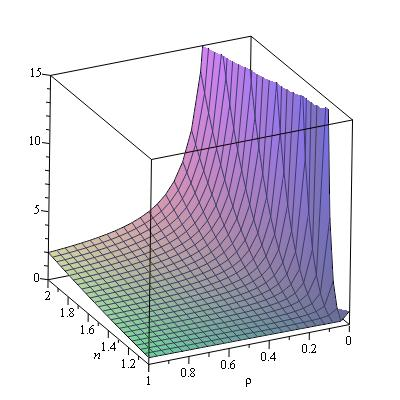
\includegraphics[width=0.7\columnwidth]{ChapterEcon/figures/integralCES}%
\caption{Continuous CES function, $0<\rho<1$, $1<n<2$; n is the number of varieties. Vertical axis shows utility.}%
\label{fig:CESintegral}%
\end{figure}

Whereas $F$ is straightforwardly the quantity of food, $M$ is actually \emph{the utility from manufactured goods}, not the quantity consumed. Intuitively, it is obvious that a single value $M$ could not represent a range of different manufactured goods directly, but this is a potential source of confusion, since - for example in Brakman \emph{et al.} - it is sometimes described as straightforward ``consumption of manufactured goods'' (p.90). \citeauthor{fujita_spatial_2001} (p.47) label $M$ a `composite index of the consumption of manufactured goods' (ibid p.46) but also note it can ``can be thought of as a utility function''. To keep things as simple as possible, that is exactly how it will be treated here. The actual mathematical definition of $M$ is a \gls{ces} function containing each variety of consumed manufactured good, of the form described in equation \eqref{eq:-6} and repeated here. $N$ is the total number of varieties consumed; $c(i)$ is the quantity of a single variety:

\begin{equation}
M=\left(\sum_{i=1}^{N}c_{i}^{\rho}\right)^\frac{1}{\rho},(0<\rho<1)
\end{equation}

So, for a given quantity and number of goods, increasing \gls{lov} (as $\rho\rightarrow 0$) increases $M$. 

A vital assumption of the \gls{dxs} is that goods enter symmetrically into demand. As Fujita \emph{et al.} note, this ``lets us have our cake in discrete lumps while doing calculus on it, too'' (\citealt{fujita_spatial_2001} p.7). What this means in practice is that, in the many-good CES function \eqref{eq:-6}, all $c_{i}$ have the same value. Sometimes, this is guaranteed mathematically by defining it as an integral (see e.g. \citealt{fujita_spatial_2001} p.46), where $n$ is the (now continuous) number of varieties, and $m(i)$ stands in for the consumption of each variety. (Note that $M$ is still manufacturing; in the \gls{dxs}, $M$ and $F$ go into a Cobb Douglas, and so demand for each sector is independent of the other: changes in the size of $M$ cannot affect demand for $F$).

\begin{equation}
M=\left[\int_{0}^{n}m(i)^{\rho}di\right]^{1/\rho}\; 0<\rho<1\label{eq:integralCES}
\end{equation}

It helps to get a quick visualisation of what this means by reframing \eqref{eq:integralCES}, assuming one unit of each variety:

\begin{equation}
M=\left[\frac{n^{\rho+1}}{\rho+1}\right]^{1/\rho}\label{eq:integralCESsimplified}
\end{equation}

The starting point for the \gls{dxs} approach has already been outlined in discussing the \gls{ces} function. That section explained how the \gls{ces} can be used to describe an `optimum product diversity' from a utility point of view. It was explained that $\rho$ controls \gls{lov}: the closer to zero, the more variety is preferred. If the number of varieties is a continuous quantity, ranging from one to two, $\rho$ looks like figure \ref{fig:CESintegral}. $M$ increases either as $\rho$ approaches zero or as the number of varieties $n$ goes up. Where $\rho=1$, goods are perfect substitutes. In this case, it can be seen that $M$ increases linearly with $n$. As will be explained, however, the number of varieties is endogenous in the \gls{coremodel}.

The budget constraint for the \gls{repag} consuming food and manufactures is as follows, where again $c(i)$ is a single variety and $p(i)$ its cost:

\begin{equation}
F + \sum_{i=1}^{N}p_{i}c_{i} = Y\label{eq:cmbudget}
\end{equation}

The separation imposed by the Cobb Douglas applies to any pair of terms in the budget constraint, so as well as knowing that $F = 1- \delta Y$, it is also the case that $\sum_{i=1}^{N}p_{i}c_{i} = \delta Y$. This second term can be used as the budget constraint for $M$ - see below. The price of $F$  does not change endogenously in the model; it is set to one, leaving just $F$ in the budget constraint. The job of the agricultural sector is to provide demand in both regions so that it does not collapse to a point if and when manufacturing workers all move to one region. As mentioned above, in the region equation for $Y$, each region has $(\frac{1}{2})(1-\delta)$ agricultural income. It is $1-\delta$ across both regions, and this cannot change. Having positive demand in both regions serves a more prosaic role in the algorithm used to find the long-run equilbrium: it cannot `complete' without it (the iteration algorithm described in section \ref{sec:cmtoplevelstructure} is unable to reach a stable value).
%\cmt{why do I still feel like I'm missing something about the numeraire? Partly: what happens if you remove from model? Need to nail down. And seems like an odd place to discuss the point of agri in the model.}

One of the three `region equations' above is the `price index' $I$. This serves a very useful simplifying role in the \gls{coremodel}. $M$ has already been defined above as `utility from manufactures' using a \gls{ces} utility function. When $M$ is optimised by its budget constraint ($\sum_{i=1}^{N}p_{i}c_{i} = \delta Y$) it becomes possible to rearrange the optimisation\footnote{Brakman \emph{et al} (p.94-5) and Fujita \emph{et al} (p.47) piece their logic together slightly differently but (apart from the latter using integrable continuous varieties, not discrete) they arrive at the same place.} to find that $M = \frac{\delta Y}{I}$, where:

\begin{equation}
I = \left(\sum_{i=1}^{N}p_{i}^\frac{\rho}{\rho-1}\right)^\frac{\rho-1}{\rho}\label{eq:priceindex}
\end{equation}

$I$ is a function of the price of each variety, but also contains $\rho$, the \gls{lov} parameter. As Brakman \emph{et al} say, the price index is a ``mirror image'' of $M$ (p.99) where more varieties - or higher \gls{lov} - will \emph{lower} $I$. Noting again that $M = \frac{\delta Y}{I}$, it can be seen that lowering $I$ increases utility from manufacturing, as would be expected if either variety number or \gls{lov} were increased. $I$ thus roughly translates as ``what utility can I buy, given the price of manufacturing goods and my \gls{lov}?'' This definition of $I$ thus simplifies the optimal quantity of $M$ to the budget for manufacturing varieties ($\delta Y$) and the price index $I$, and nothing else. 

The equation for real wages (\ref{eq:realwage}, $w_{r}=\frac{W_{r}}{I_{r}^\delta}$) can now be explained in more detail. If $W$ is the nominal wage, the real wage is `what utility I can buy with $W$'. For the \gls{coremodel}'s whole economy, Fujita \emph{et al} use a `cost of living index' (p.48; see Brakman \emph{et al} p.99 also) to describe what it costs to buy a unit of utility: $I^\delta p_{f}^{1-\delta}$, where $p_{f}$ is the cost of food. $\delta$ sets the spend on manufactures and so $I^\delta$ separately describes the cost of a unit of utility from manufacturing. As the price of $F$ is set in the model to one and, since $1^x = 1$, the `cost of living index' for the whole model reduces to $I^\delta$. Real wages are then simply the nominal wage divided by this `cost of living index', giving total utility. Differences in utility between regions can then be used to determine where mobile workers will be attracted to.
%\cmt{On cost of living index: I'm unsure whether to write up that $F$ being `stuff' and $M$ being `utility' is confusing. Mull.}

%$I$ does not contain good quantities - only the price of each, $p_{i}$. It is otherwise a similar structure to the subutility function for $M$ in equation \eqref{eq:cmbudget}, and this is no coincidence. 
%be said to be ``the amount of utility that can be bought given good prices''. 
%The way in which wages are worked out is yet to be explained - but now $I$ is defined, it is possible to define \textbf{real wages}. As \citeauthor{fujita_spatial_2001} (p.64) explain, $\delta$ controls the share of overall expenditure on manufactured goods. 

\subsubsection{Production \label{sec:CMproduction}}
Section \ref{sec:marketstructure} explained the difference between perfect and monopolistic competition. In the \gls{coremodel}, agriculture is put in the `perfect competition' category, and made spaceless. Or rather, is it argued that no transport costs exist between regions, which amounts to the same thing economically, though each region has its own fraction of agricultural workers. 
%All of the assumptions that come with perfect competition allow $F$ to be the static numeraire for the model: linear production, workers and buyers are pricetakers (so the price of goods and wages never change and can be assumed to be one). 

Manufacturing is responsible for the model's dynamic outcomes. Two key stages occur to get to the region equations. The first, already discussed in section \ref{sec:marketstructure}, is the \gls{monocomp} outcome that changes in production scale means \textbf{changes in the number of firms}, not in an actual shift in any firms' own production function or price. (This is where the externalities take effect in the \gls{coremodel; see section \ref{sec:extsinspace}.) As Fujita \emph{et al} put it (p.52):

\begin{quote}
``the size of the market affects neither the markup of price over marginal cost nor the scale at which individual goods are produced. As a result, all scale effects work through changes in the variety of goods available.''
\end{quote}

In terms of market structure, the \gls{dxs} can guarantee that each firm only produces a single variety. \Gls{increts} take care of that: any firm producing one good will be locked in to producing it more cheaply than any other can. As a firm, it is always better to devote all of one's resources to that single product than attempt to split over more than one, since this allows full exploitation of \gls{increts}, and thus one's market power.

Because firms are locked into one product, the relation to \gls{lov} means that economies have an equilibrium number of firms, and thus varieties. Net firm profits are set to zero as an equilibrium condition, underpinned by arguing that profits attract firms, thus lowering the markup for other firms until the zero profit condition is met, and losses drive them away. 

%As discussed in section \ref{sec:marketstructure}, the number of firms and varieties are the same. 
So: one firm always produces a single variety, since no firm using economies of scale in a market where goods are differentiated can gain from producing more than one variety. Reducing changes in the market size to a growth or shrinkage in the number of firms (and thus varieties) is - as Fujita \emph{et al} note - ``a rather strange result'' (ibid). They do note that other competition effects obviously exist, but simplicity wins out: reducing market changes to firm/variety number is ``a dramatic simplification, allowing us to model cleanly issues that might otherwise seem intractable.'' As will be explained below, a key simplification is that price elasticity of demand ends up constant. Brakman \emph{et al} point out (p.96), this is ``the main advantage of the \gls{dxs} aproach''. It transforms an otherwise extremely complicated mathematical problem (the feedback between shifts in production function, output and prices) into a manageable model that, so it is argued, still captures the essential feedback mechanism that is key to understanding the core-periphery dynamic.
%\cmt{This ‘key to understanding core-periphery'. Issues to put in elsewhere: ch.4 on simplification. Does it work? What counts as ‘working?' It weird and wrong to look for empirical equivalents given the model's stated purpose (use daft assumptions to help cleanly analyse an issue?) What is a justifed assumption? Works under some conditions, not others.}
%Brakman: ``The internal economies of scale are not absent, therefore, but show up in only in a rather special way in the \gls{dxs} model of \gls{monocomp}.'' [106]

A series of simplifications then take place. The first of these is on the demand-side. In section \ref{sec:constrained}, equation \eqref{eq:CESconstrained} was given as the optimal amount of a particular good resulting from optimising a \gls{ces} function with a budget constraint. As discussed above, it is also possible to define a sub-equation, $I$, to make that optimisation more useful in the \gls{coremodel}. In the core model optimisation, using $I$ to simplify, the optimal amount for a single good is (\citealt{brakman_new_2009} p.94):
%(There is no need to use a simplification like $I$ in the agent model use of equation \eqref{eq:CESconstrained}.)

\begin{equation}
c_{j} = p_{j}^{-\epsilon}[ I^{\epsilon-1} \delta Y  ]\label{eq:optimalgoodscoremodel}
\end{equation}

\Gls{monocomp} assumes that the market is `large' - meaning that no single firm is able to effect it by changing price. Given this assumption, $I$ takes on a vital role: it contains the price choices of all other firms ($p_{i \ldots n}$) and, since a single firm is assumed unable to effect it, it can be treated as a constant (\citealt{brakman_new_2009} p.96; \citealt{fujita_spatial_2001} p.51-2), along with the split of income going to manufacturing, $\delta Y$. Brakman \emph{et al.} include the square brackets in equation \eqref{eq:optimalgoodscoremodel} to indicate that the whole term can be treated thus. So, they define $constant_{1}=[I^{\epsilon-1} \delta Y ]$. Substituting this into \eqref{eq:optimalgoodscoremodel} means the optimal output of a variety becomes the following. This definition is key to how firm profit and number are worked out next.

\begin{equation}
c_{j} = p_{j}^{-\epsilon} * constant_{1}\label{eq:optimalgoodswconstant}
\end{equation}

On the demand side, then, the optimal amount of any single good is defined. This can then be plugged into the \emph{supply} side. This is one point in the \gls{coremodel} (though not the only one; see the construction of $W$ below) at which demand and supply are linked together into a production equilibrium. The stages for this are as follows:

\begin{itemize}
\item Define the production function in terms of $l$ (the straight-line equation $l = \alpha + \beta x$): ``the amount of labour necessary to produce $x$'' (\citealt{brakman_new_2009} p.102). Brakman \emph{et al} use $x_{i}$ to label `quantity of variety $i$'. This is different from $c_{j}$ only in that the latter is the \emph{optimised} quantity of good. $\alpha$ is the fixed amount of labour required, and $\beta$ is the marginal amount. (This is equation \ref{eq:coremodelMprod} for `fixed' economies of scale, discussed in section \ref{sec:prodfuncts}.)
\item Define a firm's profits $\pi$ using the production function. Profits are equal to total takings (price times quantity) minus total outgoings (wage times amount of labour):
\end{itemize}

\begin{equation}
\pi = px - W(\alpha + \beta x)\label{eq:profits}
\end{equation}

\begin{itemize}
\item Firms want to maximise their profit. This is done by maximising the profit equation using what has been deduced about demand - thus linking optimal supply and demand. So, substitute in equation \eqref{eq:optimalgoodswconstant} (the optimal amount of good, given what economic facts firms take as constant) to replace $x$. If this altered profit equation is differentiated and set to zero, this is describes the first order point of maximum profit. Through rearrangement, it ends up as a simple optimal price equation, known as `markup pricing' (\citealt{brakman_new_2009} p.103-4). This is: 
\end{itemize}

\begin{equation}
p = \beta W / \rho\label{eq:markupprice} 
\end{equation}

\begin{itemize}
\item Given that the \gls{lov} parameter $0 < \rho < 1$, if $\rho=1$, the markup price becomes just $p=\beta W$. So, where there is no \gls{lov} and all goods are substitutes, price is equal to marginal cost. As $\rho \rightarrow 0$ and goods become increasingly differentiated, so the price each firm charges increases above marginal cost.
\item This potential for profits is where the dynamic for changing firm numbers comes from, as section \ref{sec:marketstructure} explained. Profits attract firms, losses drive them away. So if profits in equilibrium are zero, the profit equation \eqref{eq:profits} can be set to zero. Also, the optimal `markup price' has been deduced, so this can be substituted into the profit equation, replacing $p$. Optimised demand and supply are now linked, and a number of key mathematical deductions then follow that each lead on to the next.
\item First: an optimal amount of good in equilibrium is found: 
\end{itemize}

\begin{equation}
x=\alpha(\epsilon - 1)/\beta\label{eq:optgood}
\end{equation}

\begin{itemize}
Second: this optimal quantity for $x$, when plugged into the production function \eqref{eq:coremodelMprod} gives the ``amount of labour required to produce this much output'' (\citealt{brakman_new_2009} p.105): $l_{i} = \alpha \epsilon$. Lastly, the equilibrium number of firms $N$, which is just the number of manufacturing workers divided by the number required to produce one variety (since each firm makes only one variety). Taking into account that $\lambda_{1}$ and $\lambda_{2}$ describe the split of workers across two regions, it becomes $\lambda_{n} \delta / l_{i}$ or, using the full definition for $l_{i}$:
%Using the full definition for $l_{i}$:
%Note, I was changing this round because I wasn't sure whether to set it for a region. But FKV do this, labelling it $L_{m}^r$, `the number of manufacturing workers at location r'. So we do want that.

\end{itemize}

\begin{equation}
N = \lambda_{n} \delta / \alpha \epsilon\label{eq:eqfirmnumber} 
\end{equation}
%\cmt{I'm already assuming the normalisation of $\gamma=\delta$}
%\cmt{I've forgotten where \alpha \epsilon comes from. Do I need to remember? Probably not.}

As mentioned above, causally, firms follow workers in the \gls{coremodel}: their equilibrium number is a direct result of the quantity of labour and demand in a region. Fujita \emph{et al} are explicit about this as well: ``we are assuming that the entry and exit of firms occurs very fast - so profits are always zero - but relocation of workers among sectors or locations occurs more slowly, with a dynamic we model explicitly'' (\citealt{fujita_spatial_2001} p.53). The latter dynamic is the long-run equilibrium of workers moving between regions. 

\subsubsection{Piecing the `region equations' together}

The equations deduced above can now be used to build the `region equations', with one extra addition: transport costs. Before coming onto these, however, the equation for regional income $Y$ is the most straightforward of the three and easy to clear out of the way first. There is only wage income in the \gls{coremodel}: the zero-profit conditions for both sectors rule out any income for firms or owners (\citealt{brakman_new_2009} p.113). The agricultural sector is entirely static, its income set to $1-\delta/2$ for each region. Income from the manufacturing sector is just its wage $W$ in each region, times the number of manufacturing workers there: $\lambda_{n} \delta W_{n}$. $Y$ is the sum of these two: 

\begin{equation}
Y_{n}=\lambda_{n}\delta W_{n}+(\frac{1}{2})(1-\delta)\label{eq:regionincome}
\end{equation}

As already mentioned, $T$ defines the transport costs between regions\footnote{Since only the two-region \gls{coremodel} is being discussed here, $T$ does not need a subscript. Transport costs for the home region are 1, $T$ otherwise.}, having a value of one for `here' and $T>1$ for the distant region. $T$ is used to simply multiply the cost of goods, so they remain the same for `here' and have a transport markup for elsewhere. The effect on demand is described by Brakman \emph{et al.} thus (p.115): ``If there are positive transport costs, that is $T>1$, demand in region 2 for products from region 1 is lower than without transport costs, because transport costs make them more expensive.'' These transport costs can be plugged directly into equation \eqref{eq:markupprice}, the cost a firm charges for a variety: 

\begin{equation}
T p = {T \beta W /} \rho\label{eq:markuppriceplusT}
\end{equation}

Equation \eqref{eq:markuppriceplusT} is the final piece of the puzzle that allows one of the region equations, the price index $I$ (equation \ref{eq:priceindex}), to be constructed (though note that some normalisations are required to reach the versions in table \ref{tab:op_eqs_coremodel}; these are discussed below, but the result will be to leave them stripped of any values for $\alpha$, $\beta$ and $\rho$). $I$ uses a sum of the price each firm charges. Equation \eqref{eq:markuppriceplusT} can provide the price each firm charges in all regions it sells to. The equation for firm number \eqref{eq:eqfirmnumber} was given above: if $l_{i} = \alpha \epsilon$, the number of firms is $\lambda_{n} \delta / \alpha \epsilon$. As \citealt{fujita_spatial_2001} note (p.50), since all varieties in a single region have the same non-transport price, it is possible to simply multiply the number of firms by this price, for each region being sold in - meaning that equations \eqref{eq:markuppriceplusT} and \eqref{eq:eqfirmnumber} can be substituted into \eqref{eq:priceindex} to produce a value for $I$ in each region\footnote{Again, Brakman \emph{et al.} provide a note showing these two equations plugging directly into the price index (p.112). Equation \eqref{eq:regionalpriceindexunnorm} is simply an algebraic rearrangement of this, keeping $W$ and $T$ tidily in the region summation.}. This is the $n$ region version, where $I_{r}$ is the price index in region $r$ (`here') and $s$ is an index for all regions:

\begin{equation}
I_{r} = \left(\frac{\beta}{\rho}\right)\left(\frac{\delta}{\alpha\epsilon}\right)^{\frac{1}{1-\epsilon}} \left[\sum_{s=1}^{N}\lambda_{s}W_{s}^{1-\epsilon}T_{rs}^{1-\epsilon}\right]^{\frac{1}{1-\epsilon}}\label{eq:regionalpriceindexunnorm}
\end{equation}

This leaves only the regional wage $W$. This is solved by assuming supply equals demand, and working out both sides of that equation (\citealt{brakman_new_2009} p.115). Once more, this process starts by using the equation for demand for a variety \eqref{eq:optimalgoodscoremodel} and substituting. The `markup price plus transport costs' equation \eqref{eq:markuppriceplusT} stands in for price. The result describes ``demand in region $r$ for a product from region $s$'' (ibid. p.116):

\begin{equation}
x_{s} = \delta \left(\frac{\beta}{\rho}\right)^{-\epsilon} Y_{r} W_{s}^{-\epsilon} T_{rs}^{-\epsilon} I_{r}^{\epsilon-1}\label{eq:totaldemand}
\end{equation}

Equation \eqref{eq:totaldemand} is included here because the next step captures where the `iceberg' part of transport costs come in. The first thing that needs to happen is to find demand for $x_{s}$ in all regions. (Note that $W_{s}$ can be moved outside the summation as $r$ is being iterated.)

\begin{equation}
\delta \left(\frac{\beta}{\rho}\right)^{-\epsilon} W_{s}^{-\epsilon} \sum_{s=1}^{N} Y_{r} T_{rs}^{1-\epsilon} I_{r}^{\epsilon-1}\label{eq:totaldemand}
\end{equation}

As well as rearranging, the whole has been ``multiplied by $T_{rs}$ to compensate for the part that melts during transport'' (ibid). Thus, equation \eqref{eq:totaldemand} is what demand firms face, which must include the full good - hence the key difference in demand from the point of view of the consumer and the firm, seen in the difference in $T$: $T_{rs}^{-\epsilon}$ multiplied by the transport cost to include what `melts away' when consumerd is $T_{rs}^{1-\epsilon}$. Consumers get $x$, for a price $T p$ that includes the transport cost. Producers have to \emph{make} $x * T$.

The supply quantity, the `optimal amount of good in equilibrium', was already given above in equation \eqref{eq:optgood}: $\alpha(\epsilon - 1)/\beta$. In equilibrium, this must match the demand given in equation \eqref{eq:totaldemand}. The two when equated can be simplified and rearranged to give the equation for $W$ (ibid. p.117):

\begin{equation}
W_{s} = \rho\beta^{-\rho} \left(\frac{\delta}{(\epsilon-1)\alpha}\right)^{1/\epsilon}\left[ \sum_{r=1}^{R} Y_{r}T_{rs}^{1-\epsilon}I_{r}^{\epsilon-1} \right]^{1/\epsilon}\label{eq:fullWequation}
\end{equation}

\subsubsection{Normalisations \label{cm_normalisations}}

As mentioned, the \gls{coremodel} equations can be simplified by `choice of units'. As \citealt{fujita_spatial_2001} say (p.54), ``we are free to choose units of measurement - be it units, tens of units, kilos, or tons.'' Given the fact that only $\lambda$ actually has any dynamics, this leaves a lot of static variables that can be set as the modeller wants. The marginal labour requirement $\beta$ can thus be set to equal $\rho$. This has no economic meaning, but it does allow a number of simplifications. Immediately in $I_{r}$, the term $\beta/\rho$ becomes $1$ and disappears. Next, the fixed labour requirement can be set to $\alpha = \delta/\epsilon$. Again in $I_{r}$, this then allows the term $\delta/\alpha \epsilon$ to become $1$ also. This leaves $I_{r}$ as it is in table \ref{tab:op_eqs_coremodel}. 

The same two normalisations can also be used to reduce $W$ to its simpler form. This is easiest done before rearranging in terms of $W$ with the two supply and demand equations. First, the supply-side, equation \eqref{eq:optgood} $\alpha(\epsilon - 1)/\beta$ reduces to $\delta$ by first substituting $\rho$ for $\beta$ and $\epsilon-1/\epsilon$ for $\rho$, leaving $\alpha \epsilon$, then using $\alpha = \delta/\epsilon$, ending up with just $\delta$.  On the demand side, in equation \eqref{eq:totaldemand}, the term $\left(\frac{\beta}{\rho}\right)^{-\epsilon}$ also becomes $1$ and disappears. Labelling the summation as a constant and equating supply to demand, that just leaves $\delta = \delta W^{-\epsilon} C$. Isolating $W$, $\delta$ can cancel, leaving $W = C^{1/\epsilon}$. Substituting the summation back in leaves $W$ in its `region equation' form. 

One of the normalisations later added by Brakman \emph{et al.} is actually assumed to begin with by Fujita \emph{et al.}, and has already been mentioned: $\delta$ is both income for the manufacturing sector and the number of manufacturing workers. This simplification has been used throughout in order to keep the explanation as clutter-free as possible\footnote{Charles van Marrewijk provides an analysis discussing income and worker number being set to $\delta$ on the website to accompany the Brakman \emph{et al.} book. This can be found at: http://www2.econ.uu.nl/users/marrewijk/newgeo/answers/newgeo\%20answer\%203.pdf}, along with the assumption that the total number of workers is $1$. Note also, however, that using the normalisations above, the equilibrium supply quantity also became $\delta$. 
%\cmt{"Note also, however, that using the normalisations above, the equilibrium supply quantity also became $\delta$. This is a point that will be returned to in the concluding discussion to this section." Is it? I think I was going to say something about equilibrium supply being set exogenously. Need to check notes to see if important.}

The above section has pieced together the construction of the `region equations'. These equations can now be used to examine the dynamics the \gls{coremodel} is interested in. 
%The detail outlined here, however, will be returned to, both in its specifics and in how the construction process compares to the agent approach used in this thesis.

\subsection{Dynamics \label{sec:cmdynamics}}
%\begin{figure}[h]
%\centering
%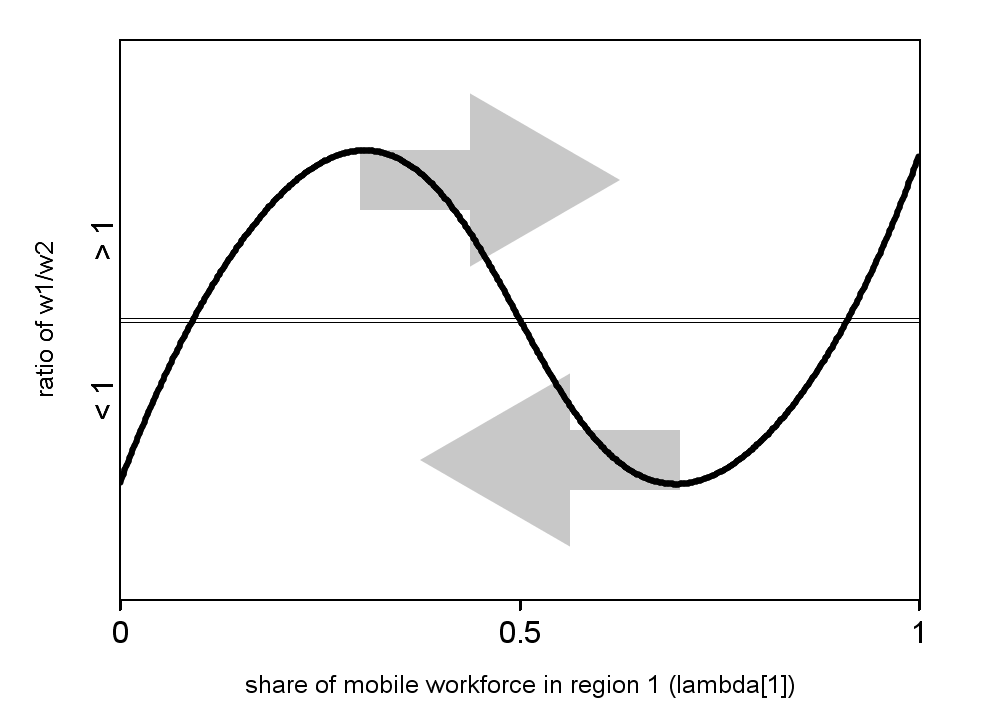
\includegraphics[width=0.95\textwidth]{ChapterEcon/figures/CMT225}}
%\caption{Short-run equilibrium. \label{fig:shortRun}}%

%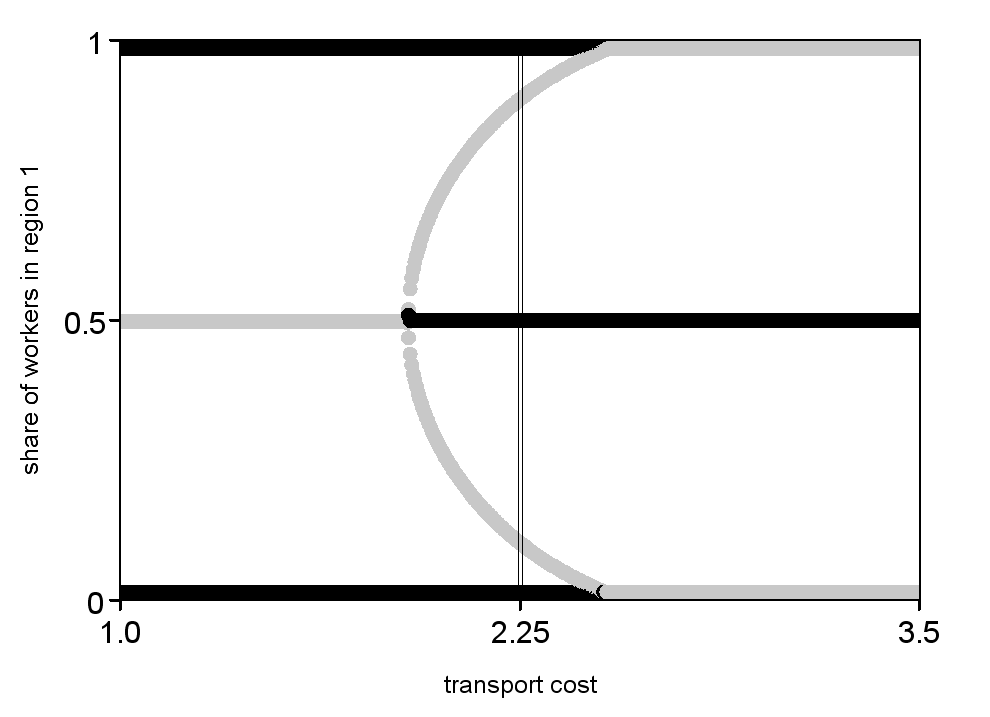
\includegraphics[width=0.95\textwidth]{ChapterEcon/figures/tomaHawk2}}
%\caption{Tomahawk \label{fig:tomaHawk}}%
%\end{figure}


\begin{figure}[p]
  \centering
  \subfloat[Short-run equilibrium]{\label{fig:shortRun}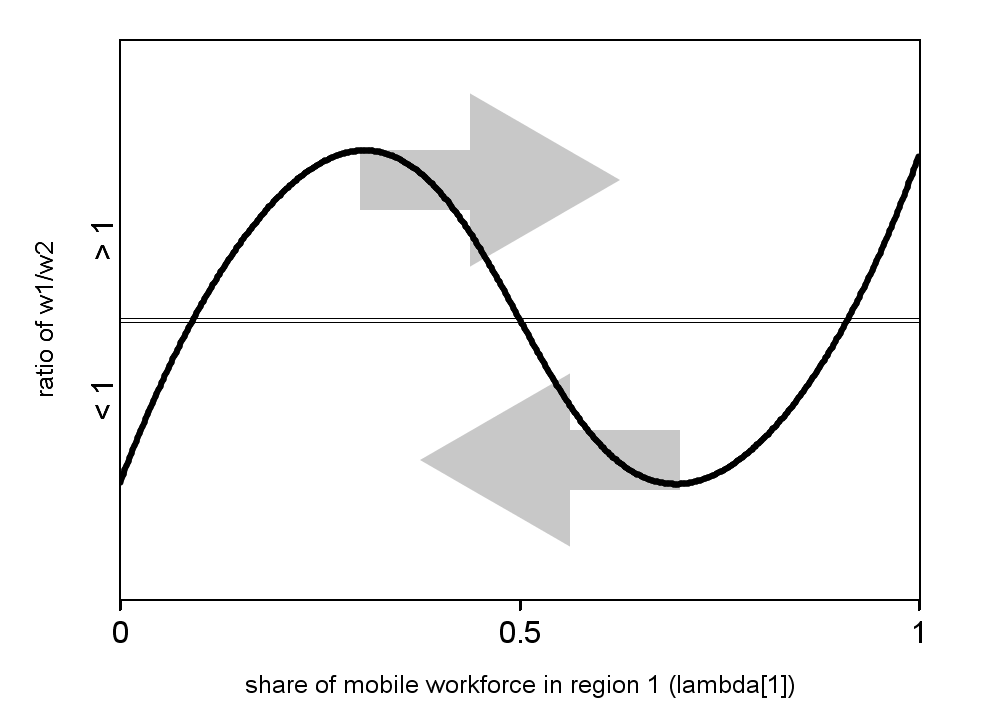
\includegraphics[width=0.95\textwidth]{ChapterEcon/figures/CMT225}}
  \hspace{0.1}    
  \subfloat[Long-run equilibria `tomahawk']{\label{fig:toma}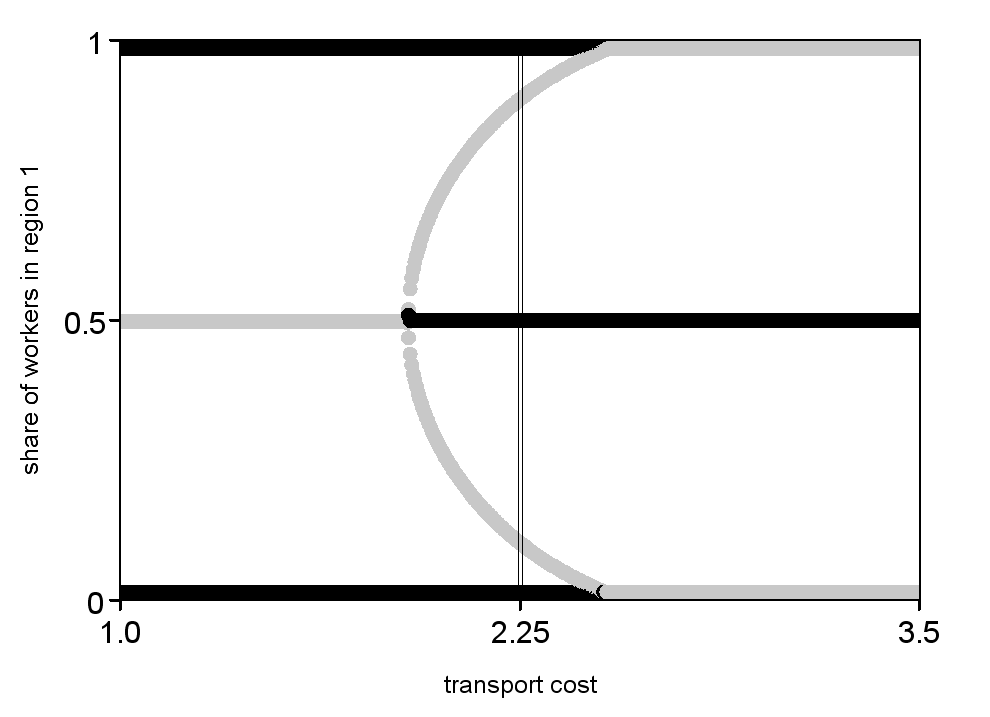
\includegraphics[width=0.95\textwidth]{ChapterEcon/figures/tomaHawk2}}
  \caption{Core model short-run equilibrium for $T=2.25$ showing real wage ratio between the two regions before migration; and long-run equilibria for $1 < T < 3.5$ showing the range of stable (black) and unstable (grey) equilibria. Double line in both crosses the same five equilibrium points for $T=2.25$. \label{fig:CMdynamics}}
\end{figure}

As section \ref{sec:cmtoplevelstructure} explained, the \gls{coremodel}'s goal is to identify a dynamic able to produce a manufacturing `core' and an isolated `periphery' using a set of simultaneous equations describing the feedback between income $Y$, a price index $I$ and the wage level $W$. That section also explained that `a simple iteration process' is used to find convergent values, resulting in a value for the real wage of each region. 

In this section, figures \ref{fig:shortRun} and \ref{fig:toma} are produced from this process, plus a second process for working out where the tension in real wages set up in the short-run leads workers to move. The figures illustrate the data in a way seen in many presentations of the \gls{coremodel}: a short-run equilibrium showing points where real wages are out of equilibrium and where they are equal and a full set of long-run equilibria for a range of transport values\footnote{Again, the commented code for producing them is available via the download link given in the code appendix (\ref{apx:modelcodeoverview}).}. 

Figure \ref{fig:shortRun} shows the first, `short run' outcome of this process for all values of $\lambda_1$ between zero and one. If $\lambda_1 = 0$ on the very left, all workers are in region two. Conversely, at $\lambda_1 = 1$, all are in region one. For each of these points, the thick black line shows the ratio of the real wage across the two regions ($w_1/w_2$). When this equals one, where the line crosses the horizontal midpoint (marked by the double line) real wages are the same in both regions. 

The vertical axis indicates that this ratio is more than one in the top half and less than one in the bottom half. When $w_1/w_2 > 1$, real wages in region one are higher: a tension is presumed to exist that will draw manufacturing workers towards region one. The direction of this tension is indicated by the grey arrow pointing to the right: any points in the upper half (where $w_1/w_2 > 1$) imply workers moving in that direction (towards $\lambda =1$). The reverse applies for the bottom half, where real wages are higher in region two. 

All other values are fixed exogenously. Manufacturing and agricultural workers are divided evenly ($\delta=0.5$). Transport costs are set to $T=2.25$. As the `long run' dynamic explanation below will show more clearly, this is in a particular part of the variable space that produces five possible equilibrium points. With the understanding that workers move to higher real-wage regions, it is possible to identify which points are stable and unstable. Where $\lambda_1=0.5$, a stable equilibrium results, evenly splitting workers between the two regions. Pushing real wages to either side of this point sets up a tension that would bring it straight back (i.e. would be `pushing against' the migration direction indicated by the arrows). Equally, the two `core' endpoints are stable - though note this is not because the ratio of real wages has equilibriated but rather because all workers have moved to that region and have no incentive to move away.

The final two points where the real wage ratio crosses the line at one are unstable. Moving an infinitesimal amount to the left of either of these points (so below the central line) implies workers moving to the left on the graph - either towards full agglomeration in region two or towards the point of even split. The same applies in reverse if the real wage shifts slightly to the right of those points.

Figure \ref{fig:toma} identifies a range of long-run equilibria showing where workers ultimately end up as they move toward higher real wages. This is done for a spread of transport values between one and $3.5$ (starting at one because, as mentioned, transport costs in the \gls{coremodel} describe `the number of goods that need to be shipped to ensure that one unit of a variety arrives'). The share of workers in region one ($\lambda_1$) is shifted onto the vertical axis. The value of $T=2.25$ used in figure \ref{fig:shortRun} is at the middle point of the horizontal axis; the double line in both figures crosses the same five equilibrium points but is on the vertical axis in figure \ref{fig:toma}.

Five hundred data points were taken across the range of transport costs and, for each of those, five hundred between $0 < \lambda_1 < 1$. Each datapoint is checked to see if it crosses the line where real wages are equal. If two points do so, they are on each side of an equilibrium. Each is then checked for stability. 

To be stable, the real wage on each side must move workers back to the same point. When does this happen? The arrows in figure \ref{fig:shortRun} help make this clear: where the ratio is more than one for the lower value of lambda (or where values drop going `left to right' in figure \ref{fig:shortRun}). For example, if $w_1/w_2 > 1$ (or real wages are higher in region one,  pushing workers `to the right' towards that region) workers will be pushed towards higher values of $\lambda$.

Black lines show where the stable equilibria are found. Grey lines show unstable equilibria (or show where all workers being present in one of the regions is not stable and will move towards a split between the two). The five equilibrium points from figure \ref{fig:shortRun} show up at $T=2.25$ as three stable and two unstable points. 

%Investigating what happens at the edge of equilibrium points is also used in section \ref{sec:lov_vs_eos} to dig into the dynamics present in the transmission belt model.
%This first `short-run' equilibrium stage sets up the tension required to make the following argument: manufacturing workers will go where real wages are highest. The actual mathematical description of this is in some senses arbitrary. Fujita, Krugman and Venables use a simple dynamic equation: a change in workers between regions is proportional to the difference between the real wage in a region and the model's average real wage. There is long-run equilibrium when this dynamic equation has reached zero. (This use of a dynamic equation to target zero is used in the model framework in a quite different way; see section \ref{sec:stocktarget}.)
\subsection{Core model: concluding thoughts}

The \gls{coremodel} is made up of a series of optimisation stages. These are, in the scaffold stages, all about finding points of no change: Lagrangians for the budget optimisations, a profit-maximisation (including some demand simplifications - the added constant term) and a zero-profit rule (built on the \gls{monocomp} argument from the \gls{dxs}) that is responsible for the equilibrium firm number. In the final `long-run' equilibria, an `ad hoc' approach moves workers to the region with the highest real wage. 

The \gls{coremodel} is the canonical example of how \gls{ge} `solves' the dependency issues of spatial economics described in section \ref{sec:spacesituate}. This section has examined in detail the way \gls{ge}'s assumptions have been implemented, providing a solid base for comparing to those of \gls{abm} and preparing the ground for explaining what components and assumptions the thesis model framework uses. 

In particular, the transmission belt model in chapter \ref{chapter:connectedModels} builds up from separate agents making their own economic decisions. It uses methods that allow asymmetric consumption of goods in order to allow a flexible way to examine different spatial setups. Also, rather than assuming increasing returns manifest through changes in the equilibrium number of firms, a model is presented that utilises increasing returns at the production level (section \ref{sec:prodtowelfare}). 

That chapter also picks up on many points covered in this section regarding particular features of the \gls{coremodel}'s assumptions and construction. This theme is taken up in depth in the conclusion, which includes a direct comparison between the \gls{coremodel} and the thesis model framework (section \ref{cmcomp}). 

\section{How space is theorised in the thesis model framework \label{sec:elementsmodel}}

This and section \ref{sec:extsinspace} concentrate specifically on the background for how `space costs' are implemented in the thesis model framework. `Space costs' is used as a top level term to describe all costs that impact on agent decisions in a spatial setting. In the thesis, there are two distinct types of space cost.  `Distance costs' are the actual costs of moving goods or people across physical distances. `Proximity costs' are used to describe any costs or benefits that arise from agents being closer to or further away from each other; these are often discussed in terms of `externalities' (see section \ref{sec:extsinspace}). Each of these has a matching section within chapter \ref{chapter:modelfw} where the specific mathematical and coding set-up for each is explained. Proximity costs, in the thesis framework, become a `density cost' that is incurred by each agent. These are covered below under three broad headings:

\begin{itemize}
	\item The cost of moving goods (connects to section \ref{sec:costmovinggoodsFramework})
	\item The cost of moving people (connects to section \ref{sec:peoplemovingFramework})
	\item The cost and benefits of proximity (connects to the density cost outline in section \ref{sec:densitycostsetupFramework})
\end{itemize}

Section \ref{sec:spacecostgoods} explains how these three are translated into the model framework itself. The final section in this chapter (section \ref{sec:spacecostissues}) examines a number of space cost issues that, while important for a full understanding of spatial economics, have been placed outside the scope of the thesis model framework. 

\subsection{Goods \label{sec:costmovinggoods}}

The thesis model framework takes a very literal approach to distance, in contrast to the `iceberg' transport costs of the \gls{coremodel} (section \ref{sec:coremodel}), where the goods themselves `melt away' and a single parameter controls ``the number of goods that need to be shipped to ensure that one unit of a variety of manufactures arrives per unit of distance'' (\citealt{brakman_new_2009} p.109). In \gls{ge}, distance is used as a broader term that can include general trade-cost impediments to the exchange of goods across space. For an \gls{abm} approach, it makes sense to treat distance in the more literal way done here, allowing actors to make decisions about specific goods with given prices.

One useful way of thinking about how this works is to consider the idea of `value density'. This can be defined as the ratio of product value to physical size or weight (\citealt{lovell_product_2005} p.144). What this idea shows is that, the more value is added, the more feasible large space costs become. That is, if a good's price is increased, the good does become more expensive - but space becomes relatively less important. Conversely, as Lovell \emph{et al.} note, ``as the value density of a product decreases the percentage of additional distribution costs increases'' (ibid.). In the models presented in section \ref{sec:results} this effect of space becoming relatively less important manifests through Peoples' spatial choices: as good costs go up, they disperse spatially.  Proximity to Firms matters to them less.

More value is added, by definition, with larger \gls{increts} (see section \ref{sec:prodfuncts}). A unit of input labour can produce a higher output. That output, however, could be measured either in added value or an increase in physical output. This is an old point of Weber's: he distinguished between processing that added weight or removed it. Lovell \emph{et al.} note Coopers' research on the production of microchips as a classic example of combining massive scale with very high value density (\citealt{cooper_logistics_1990} in \citealt{lovell_product_2005} p.144). Glaeser and Kohlhase give a good list of shipped goods with different value densities: in the U.S., wood products' average shipment length was 287 miles at their time of writing and transport costs a fifth of the value. For base metal, a tenth of the value went on transport. In contrast, machinery and electrical goods were always less than 1.2\% transport costs (\citealt{glaeser_cities_2004} p.208).

As section \ref{sec:routedev} explains, choice of transport mode is excluded from the model, but it is worth noting the relationship between value density and mode choice. As Lovell points out, it is only high value-density goods that get air-freighted (\citealt{lovell_product_2005} p.153). This highlights how important, in reality, the time element of good transport is. 

\subsection{People \label{sec:peoplemoving}}

As section \ref{sec:elementsmodelFramework} explains, the models presented in this thesis run for many timesteps, each timestep considered a `day'. People are assumed to have `one day per day' to spend and optimise using that time \textbf{only} at their point of decision. By reducing `time' decisions down to single-day optimisations, no agent is required to make any calculations involving other time periods. This is a simplification compared to real time-based decisions spread over shorter or longer timespans. In reality, real-world freight shipment happens over many days, weeks and even months and can be modelled accordingly (see, for example, \citealt{hummels_time_2001}). It also underpins problems of risk and uncertainty in trade across space (see section \ref{sec:spacerisk}). 

There are two rationales for giving agents this simple conception of time. The first is the primacy of time for the decisions people take about space - for example, the relationship between home location and commuting times. The second is that time is unique, in that an uninterrupted flow is given freely to actors, at exactly the same constant rate. It is exogenous to production and space. Equally, once used - either `spent' on space or production - it `melts away'. Most of the models presented here give actors a constant `fixed income' in this way; this can equally be considered as a fixed daily income or a `free gift' flow of time to optimise. If there is an intermediary stage of acquiring a wage, it still needs to be bought with time. 

The cost of moving people - and especially the time cost - has become increasingly the most important space cost. This is an argument made most forcibly by Glaeser (\citealt{ glaeser_cities_2004}, \citealt{ glaeser_cities_2008}; see also \citealt{beckmann_lectures_2010}, p.3). The reason is intuitive enough: as transport costs for goods drop, people's time becomes relatively more important. A knock-on consequence has been to emphasise those elements of human productivity that rely on time proximity. Leamer and Storper explain this by pointing out that -

\begin{quote}
``humans remain the containers for shipping complex uncodifiable information. The time costs of shipping these containers is on the rise because of congestion on the roads and in the airports while the financial costs of so doing are also rising due to increases in real wages of knowledge workers who are the human containers'' (\citealt{leamer_economy_2001} p.648).  
\end{quote}

The spatial consequences of this are most strongly felt for those activities requiring the most time - and employment tops this list. Close seconds are access to housing and goods. The spatial solution to this problem does not necessarily require people to stay within a day's radius: Ojo, for example, studied agricultural `commuters' in 1970s Yorubaland who developed a ``fortnightly pattern of periodic commuting to reduce the friction of distance'', moving between more distant settlements (\citealt{ojo_journey_1973} p.86; \citealt{chapman_people_1979} p.122). Closer to home, commute patterns that span larger distances than one day's range are not uncommon, but the vast majority keep to the geographical limit bounded by feasible daily commute times.

The cost of moving people is of paramount importance to firms; the idea of external costs (see section \ref{sec:extsinspace}) comes in particularly useful here. Firms face these costs from people travelling to work or moving to get goods and services. Firms primarily want to locate near to labour: as well as being intuitively obvious, this is a key finding from the literature. For instance, ``using the same workers is approximately eight times more likely to increase the degree of co-location than are trade relationships'' (\citealt{glaeser_cities_2004} p.223).  Similarly, service providers are usually reliant on proximity to customers. In both cases, the same \emph{type} of space cost exists: that incurred by people moving location. A simple example would be a hairdresser: the service provider has externalised one of the major costs - getting the person's head under the scissors from some distance away. In the case of commuting, the cost is less cleanly external or internal to the firm's production structure, since wages in part must cover it. (Section \ref{sec:firmsLoV} has an example of such an external cost and how two firms cope with them.)

For people, the direct financial cost of transport is very high, relative to how much it costs firms to move goods. Button finds that ``after housing and food, transport represents, at about 10 to 15 percent for a single-car-owning household, the largest element of expenditure out of income in industrialised countries'' (\citealt{button_transport_2010} p.90). In the U.S., Glaeser and Kohlhase note both the money and non-money movement costs people face: they cite a 2001 consumer expenditure survey showing that, in the U.S., ``18\% of total expenditures for the average household is spent on vehicle purchases, gasoline and other vehicular expenses'' - but point out that time costs are not accounted for in that, and that ``these time costs are not withering away with technological progress'' (\citealt{glaeser_cities_2004} p.208). 
%tie to theory of people as productive units.
%The precise nature of these human time-proximity effects are harder to pin down; see the discussion of localisation externalities below. 
%The cost of moving people is a particularly thorny tangle of distance and proximity costs; this is discussed in more detail in several sections below.

\subsection{The interaction of people and goods \label{sec:peopleInteraction}}

The most obvious difference between moving people and goods is the distance they cover. The prominence of time-cost for people dominates. (As mentioned, while time is a key cost for moving goods in reality, here the time element of good movement is ignored.) Good movement also does not impose the same hard limit as commuting: distance means smaller demand, but not necessarily zero demand. The geographical result of these differences is an economic landscape adapted to minimise both people-costs and good-costs into a series of overlapping plates of economic activity: Isard's `gestalt whole' (see introduction). 
%As Isard put it:
%\begin{quote}
%``Each individual commodity market including its labour, capital and land orientation possesses a particular structure which offers a certain resistance to change. Some change frequently, others slowly. Some are active, others highly inactive. By definition those markets of a relatively permanent nature, of persistent inactivity, are grouped together as the essential ones... Their combined structure determines the basic structure of the Gestalt whole, of the space economy under question.'' (\citealt{isard_location_1956} p.39)
%\end{quote}

This connects to the problem of analysing the complete impact of costs, not just those that can be measured - a point made by Burstein \emph{et al.}, who note that concentrating just on incurred costs is - 

\begin{quote}
`` - likely to underestimate true transportation costs. This is because we do not observe the cases in which transportation costs were so high that the transaction did not take place.'' (\citealt{burstein_distribution_2003} p.1198)
\end{quote}

While this problem is easy to state, it is harder to work out how those costs could be quantified. After all, it is essentially a counterfactual: what trades would have taken place if costs were lower or demand higher? The fact remains, however, that the observable situation is one where cost minimisation has already taken place. There is an overlap here with the idea of `demand thresholds', where high costs cut off transactions (\citealt{chapman_people_1979} p.86).  This has tended to be applied to consumer demand problems, rather than the economy as a whole. It is certainly easiest to understand Burstein's point by applying it to people: as discussed above, time thresholds mark a clear limit on how far people can travel to work (without needing some strategy to get around the day's time limit). The same applies to firm inputs other than labour, however. Value density and demand combine to limit the feasible range any good can be traded. 
%One possible solution is to compare the difference that cost changes make in a model; this is done in section \ref{sec:testspace}.

%This is an advantage of using the \gls{ces} function in a spatial setting to describe actual good movements (as well as labour movement in chapter \ref{chapter:connectedModels}): it is possible to examine marginal spatial changes in the abstract, avoiding the kinds of `counterfactual' 

The size of the ratio of space costs to other costs is an important determinant for actor outcomes. Consider the service industry: Glaeser and Kohlhase correctly point out that since ``transportation costs for people are still high, but transportation costs for goods are not'' (\citealt{glaeser_cities_2004} p.220), proximity to people is the most important spatial factor for services. They also note (p.201) that ``services tend to involve little freight shipment''. But what about transport costs as a proportion of the service sectors' overall costs? For the U.K. at least, Diamond and Spence found they were 9.9\%, compared to 4.7\% in manufacturing (\citealt{diamond_infrastructure_1989} in \citealt{button_transport_2010} p.58). Unsurprisingly, much of the service sector has lower overheads than other sectors. The paradoxical result is that services are more space cost sensitive. 

The introduction began with Glaeser and Kolhase claiming that ``it is better to assume that moving goods is essentially costless than to assume that moving goods is an important component of the production process'' (\citealt{glaeser_cities_2004}, p.199). They are certainly right about the relative change in importance for time versus other space costs, but assuming away those other space costs is a large step to take. 

This point overlaps with the `ecological criticism' discussed in section \ref{sec:ecocrit}: it seems, mathematically, that the importance of transport costs can be reduced simply by \emp{increasing} the cost of other inputs into the production process. By making other inputs more valuable, the importance of space can be lessened, with no limit on how much they can be reduced. 

A spatial version of the ecological criticism might go like this: it is obviously nonsense to think that distance costs can be reduced to nearly zero simply by increasing the value of other inputs. First, there are hard cost limits to moving goods and people. Second, economic value cannot be magically conjured out of thin air; as Daly put it, one cannot simply `stir faster in a bigger bowl'. Space is a crucial ingredient. Exactly how little of that ingredient is required? This problem is central to recent attempts to find ways of `decoupling' transport and economic productivity. Decoupling can be defined as ``achieving economic development without a proportional increase in transport activity (and emissions)” (\citealt{gray_decoupling_2006} p.3). Historically these two have been umbilically linked (\citealt{echenique_separating_2002}) and, while there is evidence that transport intensity (amount of transport per unit of GDP) has been dropping in the richest countries, an attendant increase in demand for oil in developing countries suggests that outsourcing of high-intensity activities is at least partly responsible (\citealt{roberts_oil_2010} p.29). 

As chapter \ref{chapter:ABM} discusses, there are no easy routes to dismissing Glaeser's simplifying assumptions out of hand as ``unacceptably distorted'' (\citealt{granovetter_sociology_2001} p.9). But ruling out non-time space costs in this way appears to also rule out asking, `what happens when they change?' It also makes it difficult, if not impossible, to investigate the relationship between space costs and productivity. 

\section{The costs and benefits of proximity \label{sec:extsinspace}}

This section explains the rationale for the `density cost' approach used in the thesis model framework. The implementation of the density cost itself is described in section \ref{sec:densitycostsetupFramework}. As the density cost results explain (section \ref{sec:results}), the density cost allows agents' decisions to accrete through external interactions or `externalities'. The meaning of `externalities' and their place in spatial economics is discussed first. The density cost is used as a proxy for a `basket' of proximity costs including congestion and land costs; this idea is discussed in section \ref{sec:landcostcong}. Finally, section \ref{sec:1st2ndnature} explains the idiosyncratically agent-based way in which `second nature', spatially relative density costs are theorised.

\subsection{Externalities \label{sec:externalities}}

Externalities have a central role to play in analytic approaches to spatial economics. Section \ref{sec:externalitiesspace} looks in more depth at the way externalities are used to define the costs and benefits of being in a specific place. The rest of this section looks at the idea itself in more detail. Button defines externalities as where - 

\begin{quote}
``... the activities of one group affect the welfare of another group without any payment or compensation being made.'' (Button 2010, p.161) 
\end{quote}
%The idea is so central for modern location theory that 'localisation' and 'urbanisation' externalities are often taken to be synonymous with agglomeration effects. 
%\cmt{vague statement about externalities being synonymous with agglom. Needs backup.}
%Indeed, the spatial equilibria that result in cities and settlements can be said to be nothing more than the balance of positive and negative externalities. 

The concept of externalities is so central because of the role they play in market structure. The pivotal chunk of Button's definition is `without any payment or compensation being made'; externalities are outside of the price system. Scitovsky (\citeyear{scitovsky_two_1954}) first clearly formulated their meaning as `direct interdependence' between economic actors. Scitovsky defined this interdependence in two ways, as technological (or `pure') and pecuniary externalities. The first, technological, he defined in relation to a firm's production function -

\begin{equation}
x_{1}=f(l_{1},c_{1},...;x_{2},l_{2,}c_{2},...)\label{eq:scit1}
\end{equation}

 - where $x_{1}$ is its output (\citealt{scitovsky_two_1954} p.145). $l_{1}$ and $c_{1}$ are its own inputs. By including a second firm's output ($x_{2}$) and its inputs ($l_{2}$ and $c_{2}$), Scitovsky explicitly states the interdependence: any alteration in the second firm's outputs or inputs will impact on the output of the first, changing the technical relations in its own production function. It is more common in spatial settings for externalities to be considered as an aggregrate effect within a region; for example, in Brakman \emph{et al.} (\citeyear{brakman_new_2009} p.38), where ``an increase in \emph{industry-wide} output alters the technological relationship between inputs and output for each individual firm. It therefore has an impact on the firm's production function'' (emphasis added). This is how external economies work, then: a firm's production function is dependent not only on the inputs it buys, but the actions of other firms. Early on, Scitovsky pointed out the rarity of this kind of `pure' externality: 

\begin{quote}
``It is not easy to find examples from industry. Going through the many examples of external economies quoted in the literature, I found only two that fit the above definition: the case in which a firm benefits from the labour market created by the establishment of other firms and that in which several firms use a resource which is free but limited in supply.'' (p.145) 
\end{quote}

Examples of the latter he gives are all common pool resources: oil-well production changes due to others drilling nearby; fishermen using the same waters; congestion problems on a public road. As he notes, even labour market pooling can be seen as a common-pool resource.

Moving on to the second type, in similar fashion, Scitovsky defines pecuniary externalities in relation to a firm's profits (\citealt{scitovsky_two_1954} p.146):

\begin{equation}
P_{1}=g(x_{1,}l_{1},c_{1},...;x_{2},l_{2,}c_{2},...)\label{eq:scit2}
\end{equation}

These profits are, of course, a function of its output and inputs, but also of other firms'. These affect the \emph{profits}, however; they do not alter the production function. Scitovsky's example of a pecuniary externality is the effect a firm's own investment decisions can have on others. One firm investing to increase its efficiency, for example, could give it better economies of scale; it can sell its output for less. Inputs to the firm increase as a consequence - this is where a pecuniary externality can be found. That increase in demand will push the price of that input up. For other firms using it, that is a negative externality. For any firms selling it, it is positive (Scitovsky p.149).

Scitovsky points out that externalities are - for general equilibrium theory and many arguments about market structure - ``the villain of the piece and the cause for conflict between private profit and social benefit'' (\citealt{scitovsky_two_1954} p.144). One of the key elements of \gls{ge}'s success stems from having managed to combine externalities and equilibrium in a way that avoids this apparent villainy.

For each of the model types in this thesis, externalities play a role. The outcome of the density cost is a form of externality caused by one Person's decisions impacting the choice set of the next (section \ref{sec:rationalchoices}). The two-Firm \gls{dmr} model (section \ref{sec:mobFirms}) examines the problem Firms have distinguishing the effect of their own action from that of another Firm - another externality. The transmission belt model's equilibrium outcome is based on price signal adjustments causing both internal and external demand effects (chapter \ref{chapter:connectedModels}). 
%More generally, it could be argued that the nature of \gls{abm} is all about externalities: an actor's choices can hurt or benefit others with no compensation being made. In those situations, the externalities do not enter into actors' functions in quite the literal way that Scitovsky describes them, but it is still useful to think about the problem from an `externality' point of view. 

\subsection{Externalities and proximity \label{sec:externalitiesspace}}

The obvious benefit of proximity is a simple cost saving: being closer means less distance to cover. This is a point often absent from discussions of space costs. Black and Henderson (\citeyear{black_spatial_1999}, p.327) are one of the few to explicitly mention it: ``capital good plants agglomerate in locations with high manufacturing employment even though this generates no externalities: it just conserves on transport costs of exchange.'' More usually, the costs and benefits of proximity are described using the language of externalities. This is how the key dynamic of the \gls{coremodel} is often framed: the effect of workers choosing to move to one region is to trigger an externality as demand for goods shifts the production structure.

This kind of regional `localisation externality'\footnote{The terminology used varies widely and can be confusing. These are agglomeration effects (sometimes described in the literature as `localisation externalities' or `localisation economies'; e.g. \citealt{malmberg_elusive_2002}, \citealt{wheeler_localization_2007}, \citealt{figueiredo_localization_2009}). Glaeser talks of `agglomeration economies' that ``exist whenever people become more productive through proximity to others'' (\citealt{glaeser_cities_2008} p.5). Again, by the definition used here, these are agglomeration effects.  There are many different terms for the opposite of agglomeration: classically, Weber used `deglomeration' (\citealt{weber_theory_1909}); Krugman uses centrifugal forces, opposed to centripetal forces holding places together; Brakman \emph{et al.} (\citeyear{brakman_new_2009}) use `spreading'. This thesis will use dispersion, following Fujita and Thisse (\citeyear{fujita_agglomeration_2002}).} 
is an effect that derives from being `here', and can be either a cost or benefit. In much of the literature (and in the \gls{coremodel}) `here' is a discrete place, which actors are either inside or out. Section \ref{sec:externalities} explained that externalities can be defined by introducing external values directly into an actors' utility or production function, or introducing them after these - for example, into a firm's income level. In a discrete space, external economies are easily implemented. For instance, in a two-region model with regions $r$ and $s$, firms in $r$ could include in their production function the total output of other firms in that region, $nx$. Using Scitovsky's way of defining an externality, that would be:

\begin{equation}
x_{r}=F(l_{1},c_{1},...;nx)\label{eq:locext1}
\end{equation}

In Scitovsky's terms, this is a pure externality since it enters directly into the production function. Economically, what does it mean? The classic example goes back to Marshall: the number of firms of the same industry in one locality increases the stock of knowledge for all firms there. This can be explained in terms of the number of workers in a region also; their presence acts as a knowledge multiplier as they move between firms. (See e.g. \citealt{ krugman_geography_1991} pp.36, and Marshall himself, \citeyear{ marshall_principles_1895} pp.349.)

These `Marshall externalities' are often contrasted to `Jacobs externalities'. These attempt to capture the central thrust of Jane Jacobs' argument: that diversity of production lies at the heart of regional productivity (\citealt{jacobs_economy_1970}, \citeyear{jacobs_cities_1986}). A simple way of achieving this would be to insert a CES-type function into \eqref{eq:locext1} rather than the raw number of firms: a region's productivity could thus, in effect, have a `love of variety'. Duranton and Puga (\citeyear{duranton_micro-foundations_2003} pp.4) use a more sophisticated version of this to model a region's gain from sharing a variety of intermediate inputs. The effect of competition between firms can also be reduced to an externality in the same way (again, as it is in the \gls{coremodel}; section \ref{sec:CMproduction}).

The common element to all localisation externalities is mathematically describing a relation to help explain the effect of many actors being in close proximity. Doing this for discrete regions has clear advantages. The effect of proximity is definable in a tidy way. One of the clearest benefits of this is empirical comparability. Being able to define a direct mathematical relationship between regional output or diversity and overall firm levels gives a simple route to regression analysis - a fact used by Glaeser \emph{et al.} (\citeyear{glaeser_growth_1992}) to identify Jacobs externalities as the most powerful (a result since challenged by \citealt{van_der_panne_agglomeration_2004}). 

As the next section explains, this thesis uses a `density cost' that, as the name suggests, is not based on a discrete absence or presence of other economic actors. The rest of this section looks at the ideas used to argue for a density cost approach. 

%A central theme examined in chapter \ref{chapter:ABM} is knowing what level of analysis is under examination, and this point is vital for discussing externalities in space. Localisation externalities can be seen as `black box' proxies for describing aggregate economic effects, supported by an argument about the market structure that underpins it. 
\subsection{Land cost and congestion \label{sec:landcostcong}}

The thesis model uses density cost as a proxy for both land costs and congestion. It is not intuitively obvious that these two can be lumped together; this section explains the argument for doing so.

Space has two fundamental kinds of cost. The first comes from distance; this has been the subject of most of this chapter so far.  Distance itself is not the cost, but rather it forces actors to spend time and resources to traverse it. It is this space that Weber worked with (\citealt{ weber_theory_1909}).

The second is productive space: land that may be bought, sold, rented and invested in, and can enter into a production or utility function as a quantity\footnote{Another common way to distinguish land components comes from eco-economics, where `Ricardian land' has both a location and `physical substrate', as distinct from its resources and productivity. This is not used here, not least because Ricardo's work on land rent was based precisely on that aspect this definition leaves out - the productive differences between types of land - rather than its location. See \citealt{daly_ecological_2003} pp.88.}. From an economic point of view, it is possible to think about land costs in the same way for farm production, factory or service output, as well as housing. Land and distance costs are of course related: this is the whole point of the von Thunen-style models described in section \ref{sec:litbits}, and can be seen in action when spatial equilibrium is discussed in section \ref{sec:results}. Where no exogenous difference in land quality is imposed, its cost must be considered as part of the other costs and benefits of being on that spot. From this point of view, a farm has the same considerations as a factory: how much land is required to produce a given output, and how does its location affect proximity to other important economic actors? This is the approach taken in the thesis.

The concept of `congestion' is broader than simple traffic-related problems. It can be used to describe a generic loss of amenity caused by density (see e.g. \citealt{glaeser_cities_2008} pp.133). Traffic congestion is an element of this, and not an insignificant one. Glaeser and Kohlhase describe the problem (for the U.S.): 

\begin{quote}
``Over the past three decades, congestion and delay have been increasing in all size classes of cities, not just the very large urban areas.  For all 75 urbanised areas taken together, on average the annual delay increased by over 280\%, with the most dramatic increase occurring for large cities - those of between one and three million - about 450 per cent.'' (\citealt{glaeser_cities_2004} p.209)
\end{quote}

The overall result from both land and congestion costs, however, is the same: higher density is expensive. This idea underpins the use of a density cost as a proxy for a range of proximity effects. As mentioned above, section \ref{sec:results} looks specifically at the outcome of this, showing that spatial equilibrium dynamics result and suggesting that spatial costs (good movement and commuting) have an opposite morphological effect to non-spatial costs.

\subsection{First versus second nature in the density cost \label{sec:1st2ndnature}}
%“Ellison and Glaeser (1999) find that natural advantages, even when very widely defined, can predict only about 20 percent of industrial localisation.” [205]

Section \ref{sec:endog} introduced the idea of `first nature' and `second nature' effects, where `first nature' are those elements already present in the spatial economy. It was mentioned that \gls{ge} models aim to endogenise as much as possible, avoiding `first nature'. 

Analytically, first and second nature effects can be distinguished thus: first nature geography is determined by absolute location (such as a resource site or port), second nature by relative location - that is, the effect comes about through interaction between locations. But as O'Sullivan and Unwin point out, ``it is usually impossible to distinguish these effects in practice simply by observing the intensity of a process as it varies across space.'' (\citealt{osullivan_geographic_2002}, p.79) 

A stronger argument than this can be made: second nature effects necessarily lead to first nature. In \gls{ge}, this is reflected in the Myrdal-style cumulative causation the models manifest (see below). Tiny differences in initial conditions determine morphology. For agent-based models, the issue is the same: as soon as two actors have formed a proximity preference, they produce a first-nature effect: their absolute location determines subsequent timesteps, and will likely determine the best choices for other agents. 

It is impossible to distinguish first from second nature effects, almost as soon as a model has started. What that means in practice is that supplying some exogenous first nature feature at time $t$ is not all that different to allowing a second nature effect to take place between two agents -  leading, as it does, to a first nature feature at time $t+1$. In \gls{ge}, this is not so relevant: the importance of endogenous outcomes is in the initial conditions, not subsequent timesteps. For agent models, which are almost always multi-timestep, the issue is a little less clear. 
%This is a vital part of the emergent pattern resulting from the use of a `density cost' in section \ref{sec:results}.

In the `mobile People' models, this point is relevant in two ways. Firstly, section \ref{sec:blackholemodel} shows that, with no other spatial costs, People and Firms will find their way to a `black hole' outcome, locating on a single spot, reducing space costs to zero. This is used to justify fixing Firms' location. While this is a `first nature' assumption, it will be shown that Firms will locate centrally for these models\footnote{This is not the case for all types of model using the thesis model framework; it is possible for Firms to seek different locations when \gls{eosub} is high in order to gain their own market share. These outcomes are not the subject of the thesis, however; for the models presented, the assumption that Firms have already found an optimal spot is justifiable. As will be discussed a number of times, for any particular assumption, `everything depends on the problem'.} and the assumption makes the subsequent analysis more straightforward.

Secondly, land costs can be considered second nature effects in the abstract. If land itself has no exogenous differences in quality, its value results from the interaction of actors. This is perhaps obvious, but it contrasts with the intuitive idea of land being `fixed' at an absolute location, and that location determining land cost. This is taken to its logical conclusion by centering a `second nature' density cost on each Person. This provides a way to explore how agents trade proximity costs off against other costs.

%There are two points that come from this. First, actors can create first nature effects on subsequent timesteps. Model approaches emphasising endogeneity do not do anything differently, necessarily, but the emphasis on second nature masks the fact that, after even one time-step, there is no real analytic difference between supplying an exogenous geographical feature and two actors creating one endogenously. 
\section{Important spatial ideas placed outside framework \label{sec:spacecostissues}}

The next chapter, as well as discussing agent modelling in depth, tackles one of the central issues of the thesis: the role of simplifications and assumptions in model-building. `Strategic simplification' is a vital part of the model-building process and best done as consciously as possible. The comparison with the \gls{coremodel} in particular also addresses this problem. This chapter ends with three other areas that, while essential to understanding the reality of spatial economics, have been specifically left out of the thesis model framework. These choices, and other lessons from comparing model simplifications, are considered again both in the following chapter and in the conclusion.
%This list is not meant to be exhaustive, but rather to illustrate that addressing what is \emph{not} part of a particular model framework is a worthwhile task.

Distance cost (for moving both people and goods) can be theorised as having three components, separate from whatever is being moved across space. First, the raw cost involved in moving people and goods. As section \ref{sec:peoplemoving} outlined, time is a key raw cost, but others include fuel costs. Second, technology: this changes the level of raw cost required to `buy' a given unit of distance (for instance, in the choice of transport mode). Thirdly, infrastructure development, such as road and rail networks or ports, that affect both technology and raw cost.

Each of these is associated with a particular timescale in which change affects actor decisions, and changes within one feeds into the others. Raw costs are the most short-term consideration. For instance, if fuel prices change, actors will immediately alter their behaviour - though fuel is a particularly inelastic commodity, so the changes will be slight (see e.g. \citealt{goodwin_elasticities_2004}). Technology change is more medium term. Using the same example, technological responses to fuel cost change have been clearly identified: actors alter technology choices in the medium-run by changing car, fleet owners by more rapidly scrapping older vehicles while companies respond to those fuel costs by building more efficient vehicles (\citealt{brons_meta-analysis_2008}; \citealt{li_how_2008}). Short-run and long-run elasticities for fuel costs, then, are reflected immediately in how much movement actors will `buy', and then in their choice of mode and vehicle. Technological change can also open up entirely new trade doorways: for example, refrigeration for meat opened up new export markets for Argentina and New Zealand (\citealt{chapman_people_1979} p.182). In the longer-run, larger-scale technology changes blend into infrastructure development as the two co-develop. 

These kinds of medium to long-term structural and technological change are put beyond the scope of this thesis. As section \ref{sec:theend} discusses, these connect to the issue of how time and spatial economics are closely intertwined - an important area for further work. The following three sections outline the background to these `strategic simplifications', starting with the longest-term source of space cost change, infrastructure.

\subsection{Avoiding infrastructure change and networks \label{sec:routedev}}

Any fully comprehensive theory of space cost change requires a theory of endogenous infrastructure and route development, that would have to include different tranport modes and their inter-relation. These long run outcomes dominate over cost change or technological change. Andersson and Stromquist make a particularly strong claim: ``all the major transitions in the European economic systems were accompanied, or initiated by major changes in transport and communications infrastructure'' (\citealt{batten_transportation_1988} quoted in \citealt{button_transport_2010} p.421). 

In the seventies, Haggett \emph{et al.}, after a detailed look at the issue, concluded that ``there remains to be specified a comprehensive model of route development'' (\citealt{haggett_locational_1977} p.95). No such model exists today, though perhaps for good reason. Infrastructure development changes proximity between points unevenly. Transport development tends to happen between economically important sites, reducing costs between them while relatively increasing costs for others. As Fowler notes, ``uneven power relations'' are both a cause and consequence (\citealt{fowler_reexploring_2006} p.1433). Routes themselves are also part of feedbacks: it is, as Chapman says, ``equally plausible to regard transport investment as a result of a need for movement or as a generator of movement'' (\citealt{chapman_people_1979} p.230). 
%\footnote{Black muses, ``perhaps it is best to have a field whose members have skills that can be applied to contemporary problems, even if such applications slow the field's conceptual and theoretical development'' (\citealt{black_transportation:_2003} p.9)}.

The obvious modelling approach to this complexity is to avoid it altogether. This is the first (and one of the most important) simplification made in this thesis: using featureless, continuous space to avoid the complications of transport and infrastructure change. This is only in any way plausible, though, for considering short to medium-term change: time-scales where the impact of route development will be only minimally felt. It is also quite a large assumption that fixed networks can be mapped onto a Euclidean plane unproblematically: see, for example, Wilhite's work on fixed networks (\citealt{wilhite_economic_2006}) and section \ref{sec:ace}. Nevetheless, this approach has one clear advantage: it is very simple. Calculations are trivial and, as an added bonus, visualisation is straightforward and intuitively easy to grasp. This method is used in this thesis; the rest of this section, however, explores the issue, to give this approach some context. It is also returned to in the conclusion, since it represents a perfect example for thinking about model simplification versus complex reality.

Infrastructure change makes no sense in anything other than a two-dimensional space (or higher). Between or within discrete regions, it must be conceptualised as either an externality (see above) or a generic transport cost change between points. Modelling space as a one-dimensional line, the same applies: there is only one route between points. Choosing discrete space or a line, however, does not make the problem go away: it just masks the fact that this uneven change dynamic exists. If, as argued here, it is perhaps the most important long-run dynamic, this means avoiding it leads to wrong results. However, as long as routes in a two-dimensional space are presumed to be static (or near-static), it is possible to assume a mapping of any route system to a Euclidean approximation, making the analysis potentially much easier. Specifically, it becomes possible to use Euclidean distance as a reasonably accurate proxy for actual distance and space cost between points (see, for instance, \citealt{cooper_use_1983}.) 

A simple way to describe the discrepancy between route distance and straight line distance is with a `route factor' (see e.g. \citealt{chapman_people_1979} p.215; \citealt{black_transportation:_2003} p.68). This is simply the ratio of the distance between points along a network route over the Euclidean distance between those points. This value approaches one as the two measurements converge, implying network density is increasing - and Euclidean approximations can do a better job. There is a well-established correlation between network density and development levels (\citealt{chapman_people_1979} p.220), and this is reflected in the route factor: it approaches one in more developed countries  - though even that assumption breaks down at small enough scales.

Early research in this area captured the most extreme manifestation of how competing interests determine route development, describing `colonial' transport networks in less developed countries. Argentina and Uruguay had railways for shipping meat and wool to Britain; Chile, Bolivia and Peru for copper, lead and tin to the coast (\citealt{gilbert_latin_1974} in \citealt{chapman_people_1979} p.231). Melchior found that ``Latin America appears as a complex of national space more closely tied to exogenous decision-making centres than to itself'' (\citealt{ melchior_integration_1972} p.88 in ibid p.16). World Bank projects still emphasise export infrastructure. 

Haggett \emph{et al.}'s work used network analysis, and this is still a common approach. Network analysis itself is, of course, now a very large part of the economics literature (for an overview, see e.g. \citealt{goyal_connections:_2009}) and has a central role in the development of complexity approaches to economics (see section \ref{sec:ace}). There is also network-related discussion in the \gls{ge} literature, but again, its focus is on \emph{economic}, not spatial or transport, networks; for example, see Johansson and Quigley (\citeyear{johansson_agglomeration_2003}), which discusses the relation of networks to localisation externalities.

More abstract network analysis relevant to transport optimisation has found an enthusiastic research community in physicists and statisticians. A particularly good recent example of this is Gastner and Newman's network growth model (\citealt{gastner_shape_2006}), in which they explicitly look for the balance between shortest routes and total route distance (that is, the sum of all route distance in the model: the more total route, the more expensive the build). They conclude that while ``these two criteria are often at odds with each other... real networks nonetheless manage to find solutions to the distribution problem that come remarkably close to being optimal in both senses'' and that `growing' them in their model does as well, or better, as attempts to explicitly optimise them. 
%The two ideal solutions were ``one which minimises the user's travel costs and one which minimises the builder's construction costs.'' [218/16] What is 'compromise' from user/builder tension?

This type of analysis, however, tends to be economics-free: cost is reduced to route length alone, and route development is not driven by particular interests. For instance, Gastner and Newman's distinction between shortest route and least total route optimisation matches the difference between optimal networks for users versus builders (\citealt{haggett_locational_1977} p.218). Users want dense networks to lower costs of travelling between points; builders want as few links as possible to reduce their costs. 

Once routes are developed, and considered as static features of the economic landscape, two types of dynamic cost are still present: arbitrage and congestion costs. (Congestion costs are discussed in section \ref{sec:landcostcong}.) The `principle of charging what the commodity will bear' applies to transport routes as any other commodity: actors will look to maximise profits (\citealt{behrens_changes_2007} p.626). This means that transport costs will, in part, reflect the fact that -

\begin{quote}
``high-value goods, for which the cost of transport will add proportionately less to total costs, usually pay more to move a given distance whereas goods of low unit value may be charged rates which do not even cover the costs involved'' (\citealt{chapman_people_1979} p.117). 
\end{quote}

Given the spatial nature of transport routes, this can often mean monopoly, monopolistic competition and cartels, as with (until recently) shipping `Conferences' (\citealt{carrere_distance_2009} p.17), American trucking prior to the Motor Carrier Act (\citealt{glaeser_cities_2004} p.204), or indeed any of the monopolised large shipping canal routes.

On static routes, the shortest route problem is quite a research topic in its own right. Discussed at length in Haggett \emph{et al.}, more recent interesting examples exist: one looks at whether supermarket delivery route optimisation can reduce the total quantity of traffic, as compared to customers driving to and from stores (\citealt{cairns_delivering_2005}). 

So, the fact that route and infrastructure development are the result of a nexus of competing interests makes any generic modelling very difficult. Euclidean space can act as a proxy in a limited way, but the above suggests that it will be less applicable in less developed countries, at smaller scales, and as longer timescales are considered. 

\subsection{Trade costs \label{sec:hiddencosts}}

Some of the most important space costs are the hardest to measure. The issue of `trade costs' is a case in point. Duranton and Storper define these as ``the sum of all costs incurred to deliver a good to its user'' (\citealt{ duranton_rising_2005} p.1)\footnote{Duranton and Storper wrote this working paper in 2005, and an article version was later published in the Canadian Journal of Economics (\citealt{duranton_rising_2008}). The original working paper has a rather more detailed introduction looking at the issue of trade costs in some depth.}. These are much broader than just transport: according to the trade cost literature, ``estimated distance effects are about an order of magnitude too large to be explained by shipping costs'' (\citealt{ disdier_puzzling_2008} p.2).  A list of potential mechanisms responsible is given by Anderson and van Wincoop: ``transportation costs (both freight costs and time costs), policy barriers (tariff and nontariff barriers), information costs, contract enforcement costs, costs associated with the use of different currencies, legal and regulatory costs, and local distribution costs (wholesale and retail)'' (\citealt{anderson_trade_2004} p.691).

The existence of trade costs are deduced by examining how trade drops off with distance between countries. Gravity models are the key tool used; an argument is then made regarding what this reveals about actors' choices. ``Theory looms large'' (\citealt{ anderson_trade_2004} p.692) - and must be made to analyse a range of costs, along a spectrum from data-rich to completely unmeasurable. The decay of trade over distance is thus - in the context of an economically grounded gravity model - taken as `revealed preference' (see section \ref{sec:rationality}). 

Using this approach has revealed an apparent puzzle: trade costs have been rising since the mid-20th century, despite transport costs dropping. Or rather, distance of trade has been dropping. Carrere \emph{et al.} conclude that if separate groups of countries are considered, distance of trade has only been dropping for poorer countries. There are two possible explanations, they argue: the lowering of trade costs between those low-income countries, or their marginalisation as trade costs with more distant countries increase (thus making nearer trade relatively less costly) (\citealt{carrere_distance_2009} p.30).

There are two closely related points relevant to this thesis. The first is the problem of mechanism: if the goal here is to model, at the actor level, decisions made given space costs, to what extent does the range of trade costs make this problematic? Any attempt to answer this question will immediately hit the second issue: what counts as an explanation of the costs identified in the real world? Section \ref{sec:levels} discusses this in more depth, as it relates to the problem of micro versus macro analysis. 

%Behrens notes that \gls{ge}  presumes ``the different components of trade costs can be reduced without loss of generality to a single parameter'' [626] and that ``the underlying assumption is that all the components of trade costs affect industry location and trade patterns in the same way.'' \citealt{behrens_changes_2007 p.626}
%(Isard is one such, and it is interesting to note that he also seems to have little time for GE-style use of transport costs: ``... it is as unjustifiable and inadequate to lump transport costs into one category along with all trade resistances in the theory of trade, as it is to treat them as implicit production costs in the theory of production'' \citealt{isard_location_1956} p.478).

%Considering all the types of dynamic that have been covered above, it is clear that many mechanisms could potentially be mechanisms underpinning trade costs. The role of network and infrastructure development in trade links has been discussed, and while Carrere \emph{et al.} pick up on the possibility of regionalised space cost changes 

\subsection{Risk is expensive \label{sec:spacerisk}}

Risk is a major cost for both firms and people, though a complex one to theorise. It is important enough for real-world outcomes that it is worth discussing briefly. Note, however, that while uncertainty does play a part, explicit risk modelling is not part of this thesis (though it is a highly interesting topic for agent modelling).

The importance of minimising risk in space costs is not new. Wallace, for example, found in the U.K. that ``where the choice between two modes involves both a considerable price and a considerable quality-of-service differential there is a clear willingness to pay the necessary price of reliability'' (\citealt{wallace_relationship_1974} p.41). Certain goods have always been more time-sensitive than others. Chapman also notes that ``consignments which fail to turn up on time impose indirect costs by interrupting production schedules. Indeed, in certain industries, the time factor is critical'' (\citealt{chapman_people_1979} p.117).

The importance of stability is clear from the way markets react to changes in the cost of oil. Price volatility is very damaging: ``not a simple dependence of the economy on the level of oil prices, as would be suggested by production-function based accounts'' (\citealt{hamilton_what_2003} p.33). This interpretation is supported by the fact that investment decisions are delayed both when oil prices increase and decrease: firm do not want to replace expensive capital at times of uncertainty. 

A more modern approach to reducing risk aversion is the trans-national corporation. As Leamer and Storper put it:

\begin{quote}
``much global trade consists merely of shipping products or components between divisions of the same firm located in different countries - transactions that do not raise the trust and enforceability issues present in arm's length transactions.'' (\citealt{leamer_economy_2001} p.649)
\end{quote}

Because of this, modern optimisation techniques for global production applied in-firm have been very successful in managing spatial risk. Carrere \emph{et al.} (discussing \citealt{abernathy_stitch_1999}) note that for apparel ``the key to success is no longer solely price competition but the ability to introduce sophisticated information links, forecasting capabilities and management systems'' (\citealt{carrere_distance_2009} p.34). This makes increasingly `lean retailing' possible, and has led to other geographical effects. Particularly, these lean firms have been bringing production networks closer: U.S. firms networked with South America and European firms with Eastern Europe - which may in part explain the trade cost puzzle mentioned above.

As with route and infrastructure development, this is a hugely important empirical area, but a particularly thorny modelling problem -  and again, one this thesis avoids. 

%Storper, agglom: Points out dropping transport costs = ‘production systems are increasingly unbundling themselves into different territories.' “Even Silicon Valley and Wall Street are now mostly the brains of far-flung input-output systems.'' [320] Note cf. ‘lean retailing', walmart, tesco, gosplan!

\section{Chapter summary}

This chapter has explained the fundamental economic and spatial economic concepts to be used in the thesis. It has placed these in the context of \gls{ge}, covering the way that market structure has been theorised. The story of how market structure assumptions have changed shows that `dependencies' in model creation are not just limited to \gls{oop}; the idea can be applied more broadly. Classical location theory ideas applicable to the thesis model framework were presented, as well as some specific classical ideas to exclude.

Time was spent laying out the exact components of the \gls{coremodel} as a way to get to the heart of the web of assumptions used by \gls{ge} and give some substance to the discussion of market structure in section \ref{sec:spacesituate}. An overview was then given of the way space costs can be theorised, looking at the costs of moving both people and goods, and the costs (and benefits) of proximity when agents are nearer together. This sets up the explanation of how these costs enter into the model framework, presented in section \ref{sec:spacecostgoods} and \ref{sec:densitycostsetupFramework}.

The chapter ended with an examination of three key issues that are consciously placed outside the analysis of the thesis, though they are discussed again in the conclusion. Throughout, a key goal has been to examine the web of assumptions in economics and spatial economics. The next chapter goes into more depth regarding the theory of assumptions in modelling and puts this in the context of \gls{abm}. The conclusion builds on this to make an argument that \gls{abm} has not yet developed an effective practical understanding of how assumptions should be understood when modelling.

\begin{comment}CUTTINZ
%As the conclusion discusses, however, it is an important area for further thought, and so it is worth specifically mentioned another theorist exl
%And then there's Hagerstrand. Or not. Decided to leave out. 
%So yes: diffusions do occur in some respects. Actually, I can connect that a little to what happens in the transmission belt model but, like the cristaller patterning, it's actually not directly relevant to the model outcomes. It does happen over time though, so perhaps worth noting. 
%Let's say: the diffusion impacts can in fact be responsible for pushing the model agents beyond their `tipping point'. But aside from the tipping point example discussed in relation to markup-seeking, the time diffusion element of this is not important for the job of this chapter, which is to examine those spaces in the model where transition between production equilibria can occur
%Isard's approach, however, was more Weberian. he argued: 
%\begin{quote}
%``Since it is the distance factor that is the heart of locational analysis, there is every reason to speak of transport inputs, wherein distance and weight are the two basic factors, and of transport rates as prices of these inputs. Location theorists unfortunately have shied away from such a concept.'' (\citealt{isard_location_1956} p.35)
%\end{quote}
%Since Isard wrote this, the `distance factor' as he describes it appears to have faded even further. 
%more basic relation to Weber is considered. Weber, Isard and \gls{ge} are all interested in the ``general laws'' determining spatial economic outcomes (\citealt{weber_editors_1909} p.xxii). The difference between a Weberian approach and that of \gls{ge} comes down to choice of abstraction. As Fujita notes (\citeyear{fujita_evolution_2010}), Isard, for one, believed that - 
%\begin{quote}
%``for a balanced treatment, the particular effects of transport and spatial costs in separating producers from each other must be considered. They are too vital to be sidestepped through implicit treatment.'' (\citealt{isard_location_1956} p.26)
%\end{quote}

Two key elements to be tested are the ability of `People' agents in the model to optimise through changing their location and the ability of `Firm' agents to do the same. Both of these present idiosyncratic challenges. A separate approach is used for each to illustrate these issues:

\begin{itemize}
	\item In section \ref{sec:results}, for investigating how `People' can optimise location and what this reveals about agent outcomes, one or more Firms are given fixed locations. For all but one result in that section, Firms are fixed at a single location and People are free to optimise their location. The result is a `monocentric' outcome (or duocentric in the case of the two fixed Firm scenario in section \ref{sec:LoVresult}).
	\item In section \ref{sec:mobFirms}, for investigating how `Firms' optimise location, People are instead given fixed, equally spaced locations along a continuous line to provide a spread of demand. Two Firms must then attempt to maximise their revenue.
\end{itemize}

%Time can thus become, if not the numeraire (see section \ref{sec:comm_costs}), then certainly a practical base for comparison.
%Fujita et al.: ``There are two main sources of evidence on this question. The first is to try to measure these costs directly, and the second comes from looking at trade volumes, and seeing how rapidly they fall off over distance'' (\citealt{fujita_spatial_2001} p.97).
%“The point is - what happens when they change?”
%Yes! That is the point! Brilliant. And of course, this separation of base and space cost as regards how actors react to density cost is perfect for that. But not very good for the larger picture, where we probably have to think about fixed positions.
%Analysing the reality of moving goods and people across space is beset by the many idiosyncracies both of these have. A particular approach has been developed for the thesis model that tries to simplify these costs into a coherent set of factors. The following sections lay out this approach, while also discussing some of the more thorny issues real-world space costs have.
%The full cost of moving goods and people goes beyond simple considerations of distance. Section \ref{sec:spacecostissues} looks at some of these considerations to give some context. The models developed for the thesis, however, do stick to examining how actors interact given simple space costs affected by distance or density. 
%That section also argues that it is possible for increasing returns to arise through \gls{lov} alone, between single actors with linear production - and so the production structure itself cannot guarantee a single good per producer. The thesis model does still use the assumption that a each firm produces a single variety; chapter \ref{chapter:ABM} discusses the problem of justifying particular assumptions in depth.
%The simplifications at the heart of the \gls{dxs} approach represent both its great strengths and its weaknesses. By building a model that reduces to so many static equilibria - and thus static parameters - a set of normalisations become possible, reducing complexity while keeping the key dynamics. Its weakness is how implausible these values can seem. \gls{ge} theorists are self-aware enough to acknowledge this. 
% - but is saying, `yes, we know this has a lot of silly assumptions' being used as a `get out of jail free' card? How to judge what is sensible and what is not? After all, the entire motivation behind the \gls{coremodel} was not to show that a core-periphery dynamic can exist - this was already known. It was to show that such a dynamic could be made to work \emph{within the neoclassical framework}. Some elements of that framework, then, are clearly indispensible, not open to being replaced with `silly' assumptions. So what makes the full \gls{coremodel} better than the very simple example using by both Krugman and Brakman? 
%Ah, they both talk about that. I'll write it down. It's something for chapter 4 as well, but worth talking about in the conclusion to wherever this section ends up.
%See FKV p.75/6 on assumptions ‘you wouldn't want to defend'. There are so many other versions of the model they try to make better - I can't learn all those, or indeed fit them in the PhD. It has be about asking what sort of model fits this idea they give: ``a model simple enough to yield readily to analysis, yet enough is going on that it yields a number of suggestive and interesting conclusions'' (p.75).


\end{comment}CUTTINZ


